\chapter{咽和喉}

\section{检查方法}

\subsection{咽部}

咽部的CT检查方法有两种:平扫和增强扫描。大部分检查需用增强扫描,以使大血管显示更清晰,有助于对病灶定性和定位,并可鉴别血管与淋巴结。同时应选用软组织窗和骨窗观察。检查以横断面为主,按需要加冠状面扫描。

1.鼻咽部:①横断面扫描:患者仰卧,以听眦线为基线,扫描范围从蝶骨平面开始至硬腭平面,层厚及间距为5mm。②增强扫描:扫描体位同上,可用100ml造影剂快速滴注,在注射总量2/3后开始扫描。③冠状面扫描:扫描基线垂直于听眦线,扫描范围从翼板前缘至第一颈椎前缘,层厚及间距为5mm。

2.口咽部:①以横断扫描为基础,扫描体位同上,从硬腭平面开始达会厌游离缘,层厚及间距为5mm。②增强扫描方法同鼻咽部。③冠状面CT检查其体位、范围与鼻咽部相仿。

3.喉咽部:用横断面扫描,可用重建图像来做冠状面成像。扫描基线与舌骨平行,范围自会厌游离缘达环状软骨下缘,层厚和间距为5mm。一般需增强扫描,方法同鼻咽部增强扫描。

\subsection{喉部}

喉部CT检查以横断面为基础,无法做冠扫。一般以薄层横断面图像做冠状面重建图。①扫描基线与声带或舌骨平行,扫描范围自会厌游离缘达环状软骨下缘。②一般层厚和间距为5mm。如欲对声带区细小病变扫描,则在声门上、下范围用2~3mm层厚作连续扫描。③螺旋CT可用2mm准直宽度,螺距1,1~2mm层厚重建,并可用仿真内镜成像。④增强扫描有利于定性、鉴别血管和淋巴结。

扫描时应注意:①受检者仰卧,下颌上抬,肩背部可安放薄棉垫。②检查时嘱患者平静缓慢呼吸,不能吞咽和讲话。③如欲了解声带活动情况可嘱受检者发“E”音,但发音时喉室位置要比平静呼吸时上提10mm左右。

\section{正常解剖和CT表现}

\subsection{咽部}

咽部可分为鼻咽、口咽及喉咽3部分。自颅底至软腭称鼻咽部,自软腭至会厌上缘(或舌骨)称口咽部,自会厌上缘至梨状窝底(或环状软骨)称喉咽部。

1.鼻咽部:位于鼻腔后方,有6个壁:①前壁为后鼻孔及鼻中隔之后缘;②顶壁呈圆形,与蝶骨体及枕骨斜坡相邻;③后壁较垂直,由枕骨斜坡和C\textsubscript{1}
、C\textsubscript{2}
及其前方的头长肌、颈长肌组成;④底壁为软腭;⑤两侧壁由肌肉和筋膜所构成。

在咽两侧壁近下鼻甲之后端各有一漏斗状开口是咽鼓管开口,在其后上方为咽鼓管软骨所形成的隆起称咽鼓管隆凸,在咽鼓管隆凸后方与后壁之间有较深的纵行窝称咽隐窝。咽隐窝上方为破裂孔,两者相距约1cm。鼻咽腔顶部有一团淋巴组织称为增殖腺(咽扁桃体),它发生于胚胎第4个月,7岁左右萎缩,14~15岁达成人状态。

2.口咽部:①前方以软腭游离缘、腭舌弓、腭咽弓和舌根等为界与口腔相通。②向下连接喉腔和喉咽部。③两侧壁有腭舌弓和腭咽弓,其间形成扁桃体窝容纳腭扁桃体。腭扁桃体与咽扁桃体、舌扁桃体和咽鼓管扁桃体、咽侧淋巴带和咽后壁淋巴滤泡共同围成一淋巴组织环称为咽淋巴内环。内环外围与颈淋巴结相互连接,形成咽淋巴外环。④后壁为
C\textsubscript{2} 、C\textsubscript{3}
椎体及其前方的头长肌及颈长肌。厚度均匀一致,成人厚约0.5cm,老年人因萎缩而较薄。⑤侧壁由咽缩肌(包括咽上、中、下缩肌)、咽提肌(位于咽缩肌内面,包括茎突咽肌、腭咽肌和咽鼓管咽肌)、腭肌(包括腭帆张肌、腭帆提肌、腭垂肌、腭舌肌)和黏膜组成。

3.喉咽部:是环绕喉腔外的间隙。喉咽由声门上喉两侧的梨状窝和环状软骨后的环后间隙(杓状软骨与环状软骨板后方的扁形腔隙)组成。

梨状窝为尖向下的三角形空腔,其各壁为:①内侧壁即声门上喉侧壁,由会厌侧缘、杓状会厌皱襞和杓状软骨组成,上缘围成喉入口;②外侧壁上段附着于舌甲膜,下段则紧贴甲状软骨翼内面;③前壁在咽会厌皱襞下反折;④后壁直接与环后间隙相连;⑤梨状窝尖可下达环杓关节外侧。

\subsection{鼻咽部横断面及冠状面CT表现}

1.横断面:鼻咽腔的形态有4种:①方形:出现在硬腭层面,其前方为腭肌,后方为颈椎前软组织,两侧为鼻咽腔侧壁。②长方形:在软腭之上层面,鼻咽腔前后径变长,呈长方形。③双梯形:咽鼓管隆凸层面呈双梯形(图\ref{fig6-1})。④梯形:咽隐窝层面呈梯形。

\begin{figure}[!htbp]
 \centering
 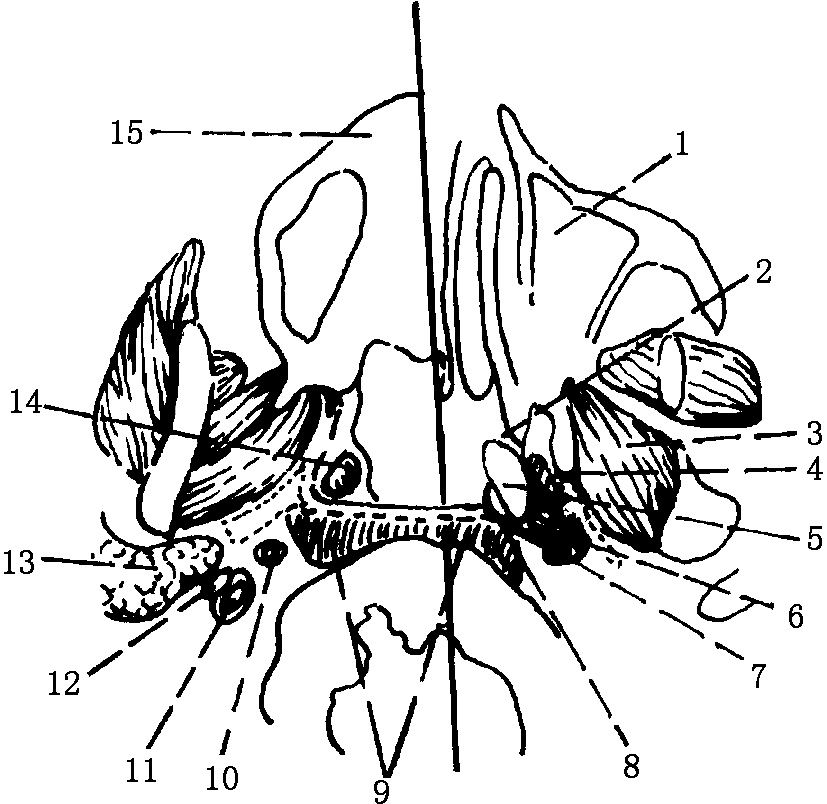
\includegraphics[width=.7\textwidth,height=\textheight,keepaspectratio]{./images/Image00134.jpg}
 \captionsetup{justification=centering}
 \caption{鼻咽部横断面\\{\small (右半图比左半图向头侧移动约1cm)}\\{\small 1.上颌窦;2.咽鼓管咽口;3.翼外肌;4.腭帆张肌;5.咽鼓管软骨;6.腭帆提肌;7.咽上缩肌;8.咽隐窝;9.头长肌和头直肌;10.颈内动脉;11.颈内静脉;12.茎突;13.腮腺深叶;14.腭帆提肌和咽鼓管咽肌;15.硬腭}}
 \label{fig6-1}
  \end{figure} 

但鼻咽腔的形态也与咽鼓管及咽隐窝是否张开有关。如果咽鼓管闭合,鼻咽腔侧壁无突出或只有轻微突出;如同时咽隐窝也闭合,鼻咽腔侧壁则变平,CT各层图像均呈长方形。如果咽隐窝轻度张开则呈梯形;只有咽隐窝及咽鼓管同时张开才呈双梯形。

咽鼓管隆凸层面是较典型的CT横断解剖图像。可见两侧半圆形凸起为咽鼓管隆凸,其前方黑色凹陷裂隙为咽鼓管咽口,其后方较宽裂隙为咽隐窝。腔后壁在中线两侧各有一圆形肌组织为头长肌,肌前方黏膜下为咽后间隙所在(正常CT扫描多不显示)。隆凸外后椭圆形肌团为腭帆提肌,该肌前外为腭帆张肌,但二肌肉与鼻咽部黏膜融和在一起,CT无法分开。

鼻咽缝间隙位于颈椎和枕骨前方并列的头长肌或颈长肌之间,咽后壁的后方,呈三角形,有时部分层面呈方形。其中间有致密的咽缝,咽缝两侧结构对称。

2.冠状面:鼻咽腔位于颅底下,顶壁软组织厚度与淋巴组织增生程度有关,成人厚约0.5~1.0cm左右,均匀对称。老年人因组织萎缩较薄,儿童因有正常或肥大增殖腺可呈块状肥厚。其侧壁可清晰显示咽鼓隆凸及其前下方的咽鼓管咽口和后上方的咽隐窝。腭帆张肌居隆凸软骨外侧,腭帆提肌居隆凸软骨下方,其下有纵行的肌束为咽上缩肌构成的鼻咽下部和口咽侧壁(图\ref{fig6-2})。

\begin{figure}[!htbp]
 \centering
 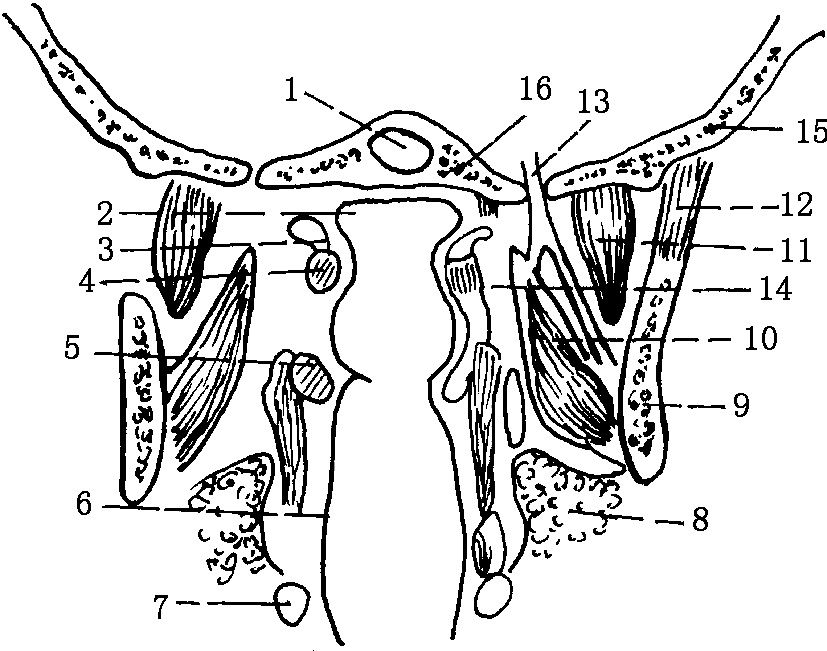
\includegraphics[width=.7\textwidth,height=\textheight,keepaspectratio]{./images/Image00135.jpg}
 \captionsetup{justification=centering}
 \caption{鼻咽部冠状面\\{\small 1.蝶窦;2.咽隐窝;3.咽鼓管隆凸;4.腭帆张肌;5.咽上缩肌;6.口咽侧壁;7.舌骨;8.颌下腺;9.下颌骨;10.翼内肌;11.翼外肌;12.颞肌;13.卵圆孔;14.咽旁间隙;15.蝶骨大翼;16.蝶骨体}}
 \label{fig6-2}
  \end{figure} 

\subsection{口咽部横断面CT表现}

口咽部上缘与鼻咽相连续,该处较狭窄称为咽峡部。其前界为软腭和腭舌弓;两侧壁为咽缩肌,其外方为透亮的咽旁间隙;后方为椎前肌组织和黏膜。软腭以下口咽腔较宽敞,呈长方形,两侧壁相对头端较厚,有时可见突向咽腔的腭扁桃体,其密度与肌组织相仿,故CT无法区分。腭扁桃体有时可见钙化斑点为炎症所致。该层面咽旁间隙亦较头端宽,在茎突内侧可见颈内动、静脉影。口咽部前部为舌背,表面有增生滤泡而使之表面不平,这些滤泡增强扫描有强化(图\ref{fig6-3})。

\begin{figure}[!htbp]
 \centering
 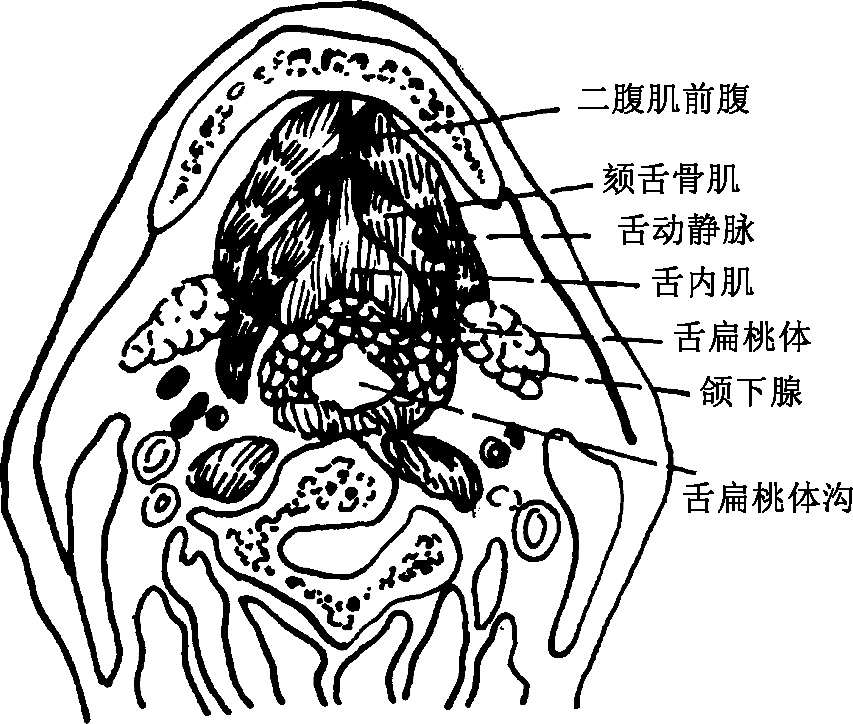
\includegraphics[width=.7\textwidth,height=\textheight,keepaspectratio]{./images/Image00136.jpg}
 \captionsetup{justification=centering}
 \caption{口咽部横断面}
 \label{fig6-3}
  \end{figure} 

\subsection{喉咽部横断面CT表现}

喉咽部横断面CT图像可同时显示喉腔。在会厌游离缘显示后,向足端层面逐渐见会厌两侧缘向后延伸,即为杓状会厌襞。该襞下延至披裂软骨。杓状会厌襞外方见一类圆形空隙即为梨状窝,该窝外壁即为咽侧壁和甲状软骨板。梨状窝上端较宽大,随发音和屏气时可扩大,其尖端和喉咽腔后部(环后间隙)正常时常呈闭合状态,故CT常无法显示。

\subsection{咽旁间隙}

该间隙是颈部最大的间隙,位于咽肌环和咀嚼肌群之间。其内侧为咽黏膜间隙,前外为咀嚼肌间隙,后外为腮腺间隙。可分为茎突前间隙和茎突后间隙,但亦有文献认为咽旁间隙仅指茎突前间隙。茎突前间隙内最主要的结构是腮腺深叶。茎突后间隙又称颈动脉间隙,内有颈内动、静脉及迷走神经等。颈内动脉居前内,颈内静脉居后外且较动脉粗大。

该间隙呈三角形,上宽下窄和后宽前窄,上端在颅底、向下达舌骨平面,由颈深筋膜反折层形成。CT横断面呈前窄后宽的三角形,前抵翼内板,后至茎突,由后外斜向前内,呈脂肪密度。老年人常较青年人宽大。

\subsection{咽后间隙}

该间隙为咽后壁颊咽筋膜(咽缩肌后面覆有颊咽筋膜)和椎前筋膜(椎前肌)之间的潜在间隙。它向上至颅底,向下达咽部和食管后面,伸延至后纵隔。间隙内为疏松结缔组织和淋巴结。其中线处有分隔将间隙分为左右两侧。该间隙内含有内、外两组淋巴结,内侧组位于中隔附近椎前肌前方,正常不显示;外侧组可突入颈动脉间隙内。

\subsection{咽黏膜间隙}

咽黏膜间隙为咽黏膜与颊咽筋膜间的潜在间隙。位于鼻咽和口咽侧壁及后壁内。主要结构为咽黏膜、淋巴组织、咽鼓管咽肌、腭帆提肌和隆突软骨。咽黏膜增强扫描呈高密度。

\subsection{咀嚼肌间隙}

咀嚼肌间隙位于颞下窝内,为颈深筋膜浅层包绕。以翼内肌后缘与咽旁间隙分开,其筋膜上延至卵圆孔内侧颅底。此间隙内包括所有咀嚼肌(翼内肌、翼外肌、颞肌、咬肌)、下颌骨支、三叉神经的下颌支和翼静脉丛等。

\subsection{喉部}

喉腔内部结构从临床角度以声带为分界线,可分成声门上区、声门区和声门下区。

1.声门上区:指声带上缘以上,上通喉入口,前壁为会厌软骨,后壁为杓状软骨,两侧壁为杓状会厌襞。介于喉入口和室带之间的喉腔称为喉前庭。室带又称假声带、前庭襞,左右各一,位于喉室上方,与声带平行。室带的前端起于甲状软骨前角中上段内面,后端止于杓状软骨前上面。位于室带和声带之间的向外突出的椭圆形腔隙称为喉室。

2.声门区:包括声带和声门裂。①声带:亦称真声带、声襞,位于喉室下方,前端起于甲状软骨前角中段内面,后端附着于杓状软骨声带突,由黏膜、声韧带和声带肌纤维组成。我国正常人声带厚约5mm;正常男性长约20~24mm,女性长约15~17mm。②声门裂:简称声门,指声带外展时,两侧声带间的喉腔裂隙,为喉最狭窄处。两侧声带前端交合处称为前联合,该处厚约1~2mm。声带后端与杓状软骨内侧之间的黏膜称为后联合。

3.声门下区:指声带下缘至环状软骨下缘以上的喉腔。

\subsection{喉软骨}

共有9块,为单个较大的会厌软骨、甲状软骨、环状软骨和成对较小的杓状(披裂)软骨、小角软骨和楔状软骨。此外,还有数目不定的麦粒软骨和籽状软骨。

1.会厌软骨:位于喉的前上部,扁平如叶瓣状,上宽下窄,在舌骨和舌根后下方,下端借甲状会厌韧带附着于甲状软骨前角内面,止于声带上缘在甲状软骨上的前附着点。很少钙化。

2.甲状软骨:由一对四边形甲状软骨板组成。成人长约4cm,高约2.4cm。前面相互融合是喉结。通常甲状软骨前角男性为直角,女性呈钝角(约
120°)。甲状软骨前角上方有“V”形凹陷称甲状软骨上切迹。甲状软骨板后上缘和后下缘分别向上、下突出称为甲状软骨上角和下角。甲状软骨可钙化、骨化并形成骨髓腔。

3.环状软骨:位于甲状软骨下方,呈“印戒”样。后面有较宽的软骨板,上下径约2~3cm;前部有狭窄的软骨弓,上下径约0.5~0.7cm。也可钙化、骨化并形成骨髓腔。前弓上缘与甲状软骨下缘之间有环甲膜相连,后板上缘两侧与杓状软骨组成环杓关节;板的两侧缘略凹与甲状软骨下角组成环甲关节。

4.杓状软骨:又称披裂软骨。呈三角锥形,左右各一,位于环状软骨板上方。其底部与环状软骨连接成环杓关节;底部前端有声带突,为声带肌和甲杓外肌附着处;底部外侧有肌突,有喉内肌(环杓后肌、环杓侧肌、杓斜肌及杓横肌和部分甲杓肌)附着。其顶的尖部伸向内后方,其上方有小角软骨,后者前外侧还有楔状软骨。

5.小角软骨、楔状软骨和麦粒软骨、籽状软骨:小角软骨呈椭圆形,楔状软骨呈小棒状,籽状软骨数目位置不定,麦粒软骨包含在甲状软骨外侧韧带中部,是胚胎期甲状软骨与舌骨连接的残余。

\subsection{喉软骨的钙化或骨化}

一般于20岁以后喉透明软骨开始钙化,50岁以后有明显钙化。环状软骨、甲状软骨和杓状软骨的大部分属于透明软骨,可产生钙化和骨化。其余喉部软骨(会厌、杓状软骨尖、甲状软骨中央部及籽状软骨)为弹力软骨,可终身不钙化。

男性甲状软骨有前后两个骨化中心,通常钙化自后下部开始向后上和沿前下部向前扩展;女性仅后部一个中心,故钙化局限于后部。钙化形态不规则。环状软骨钙化可以从环状软骨板上缘和后缘开始,向前弓上部扩展。杓状软骨底钙化在成年人中常见,CT呈对称的三角形致密影,是声带的辨认标志。

\subsection{舌骨}

舌骨出生后不久就从6个多骨化中心钙化骨化。胚胎末舌骨大角先钙化骨化,出生后舌骨体骨化,舌骨小角骨化在青春期。舌骨呈马蹄形,分为体、大角和小角。位于颈前部,以韧带与茎突相连。国内有报道,双侧舌骨大角与舌骨体间可无骨性连接而呈双侧或单侧分离,据统计竟达61%。

\subsection{会厌前间隙和喉旁间隙}

1.会厌前间隙:是位于会厌和杓会厌皱襞前的脂肪纤维组织。向下与喉旁间隙相通,向上达会厌溪。

2.喉旁间隙:是位于甲状软骨板和喉壁之间的脂肪纤维组织。真声带水平的喉旁间隙最窄,向上逐渐增宽,向上、向外与会厌前间隙相延续。

\subsection{喉肌}

喉肌属横纹肌,分为内外两组。①喉外肌:将喉与周围结构相连,主要与喉的升降运动有关,同时使喉固定。包括舌骨上肌群(二腹肌、茎突舌骨肌、下颌舌骨肌和颏舌骨肌)和舌骨下肌群(胸骨甲状肌、胸骨舌骨肌、肩胛舌骨肌及甲状舌骨肌)。②喉内肌:分为内收肌和外展肌,前者使声带内收,关闭声门裂;后者使声带外展,张开声门裂。喉内肌包括环杓后肌、环杓侧肌、杓横肌、杓斜肌、环甲肌、甲杓肌、杓会厌肌。

\subsection{喉部CT表现}

喉部CT主要通过横断面显示(图\ref{fig6-4}):



\begin{figure}[!htbp]
 \centering
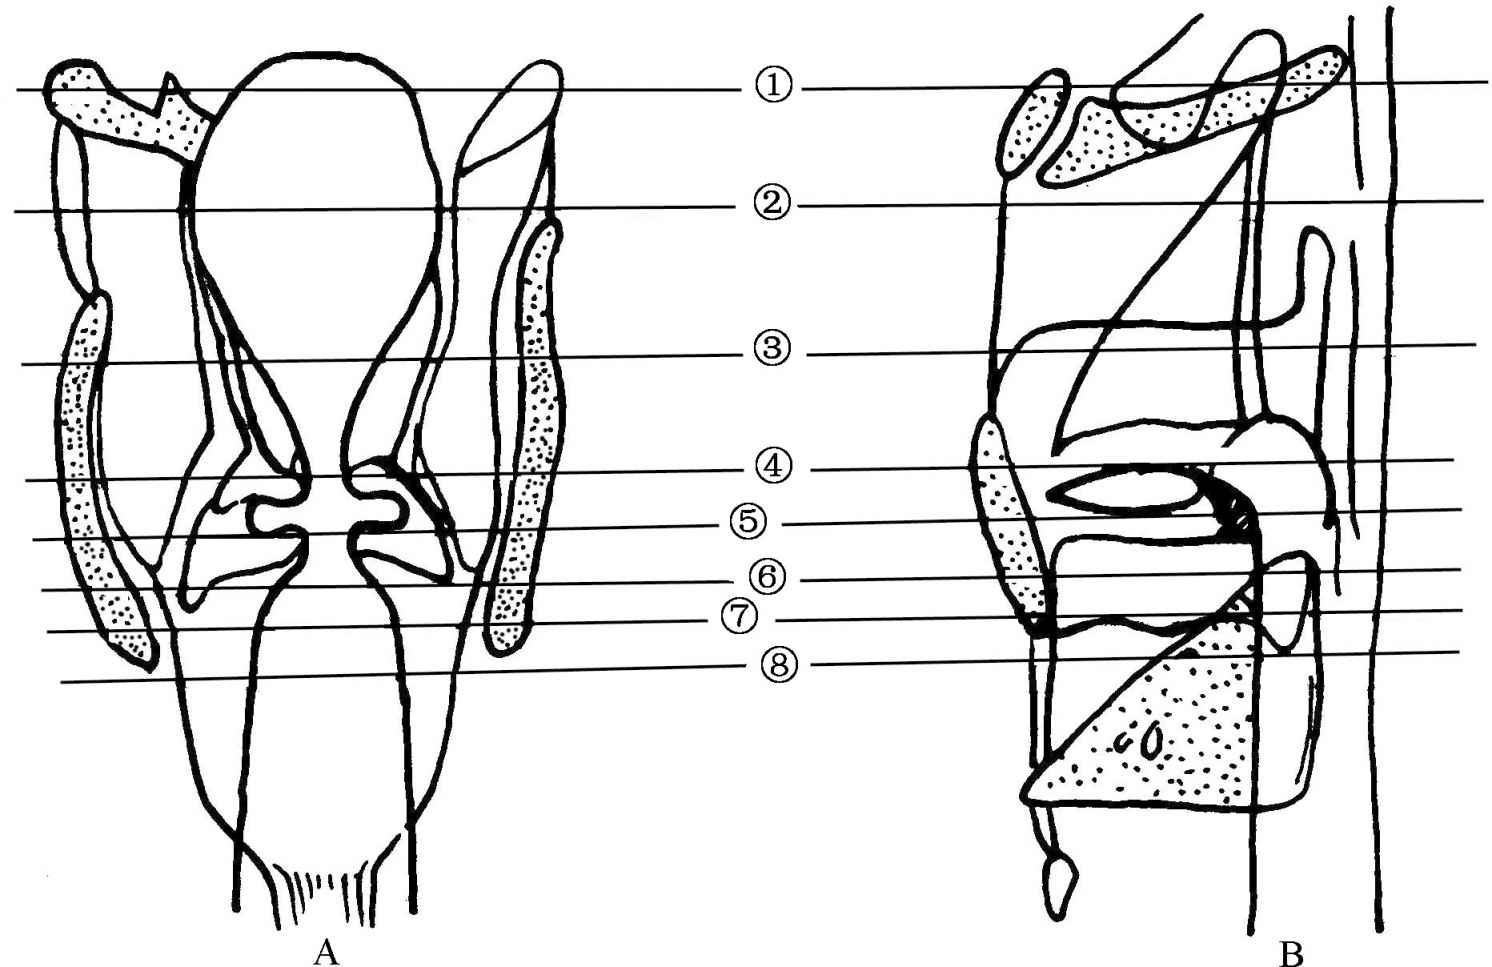
\includegraphics[width=.7\textwidth,height=\textheight,keepaspectratio]{./images/Image00137.jpg}
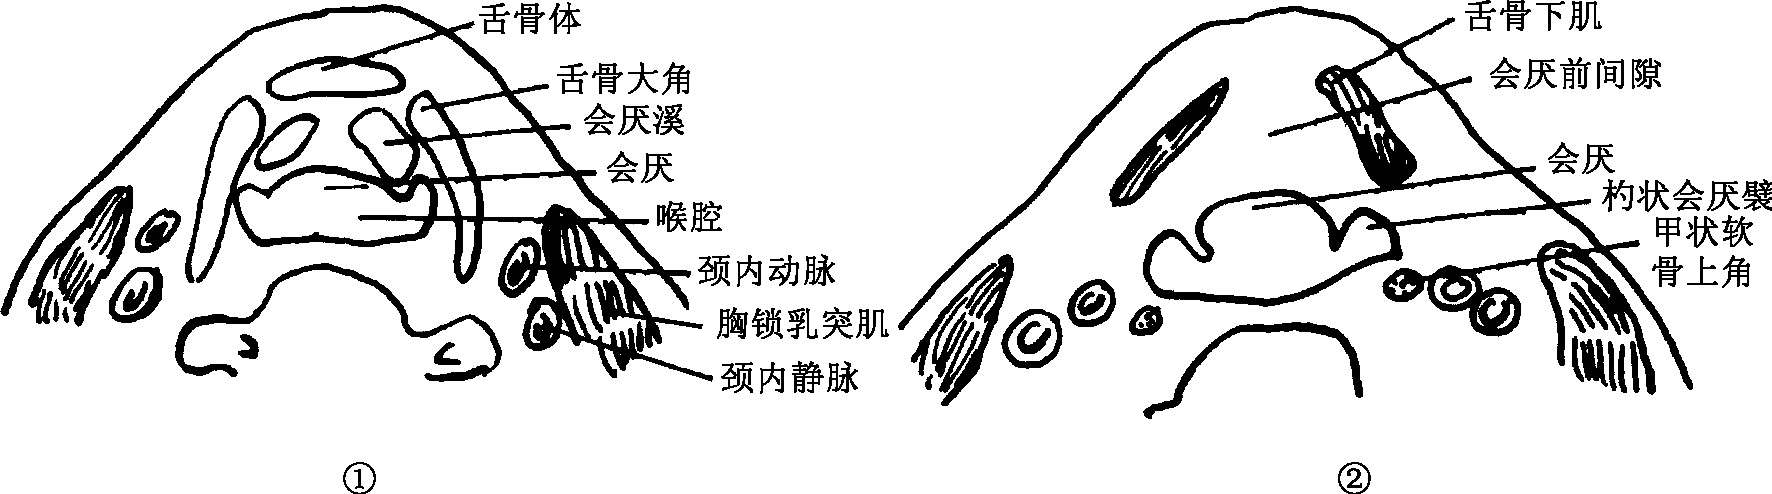
\includegraphics[width=.7\textwidth,height=\textheight,keepaspectratio]{./images/Image00138.jpg}
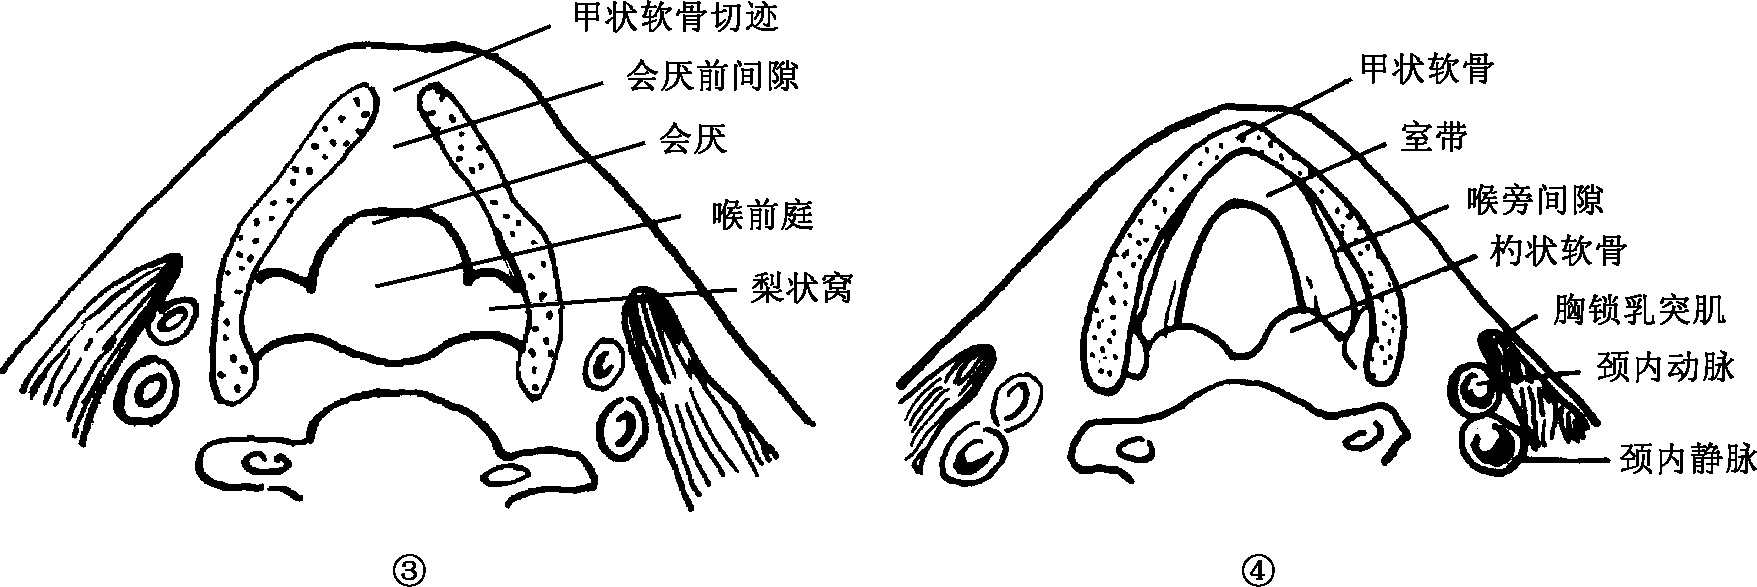
\includegraphics[width=.7\textwidth,height=\textheight,keepaspectratio]{./images/Image00139.jpg}
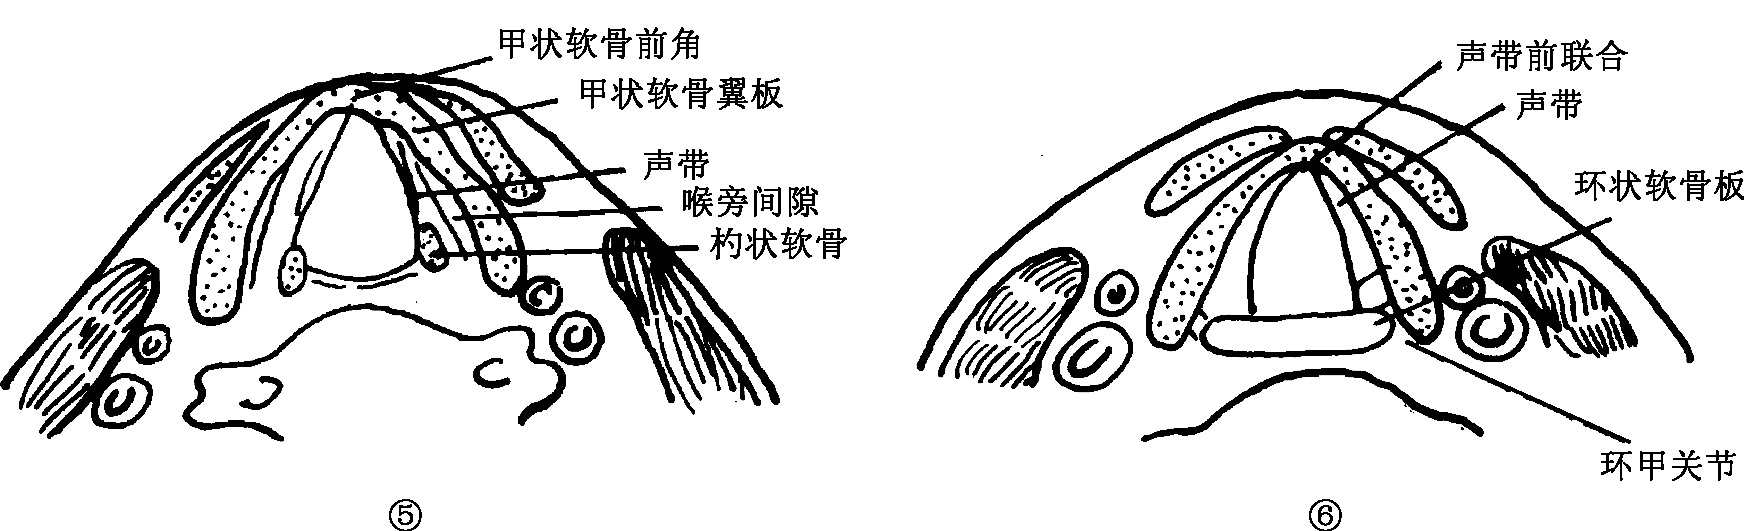
\includegraphics[width=.7\textwidth,height=\textheight,keepaspectratio]{./images/Image00140.jpg}
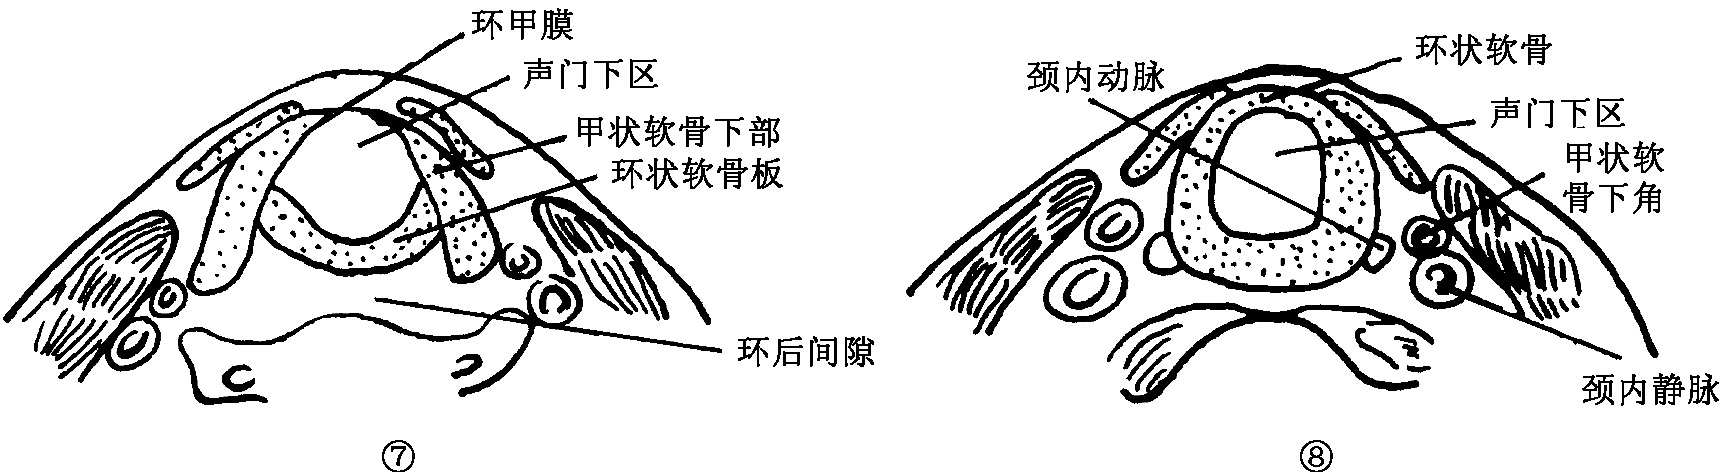
\includegraphics[width=.7\textwidth,height=\textheight,keepaspectratio]{./images/Image00141.jpg}
 \captionsetup{justification=centering}
 \caption{喉部横断面\\{\small A、B是扫描层部位;①~⑧显示各扫描层结构}}
 \label{fig6-4}
  \end{figure} 

1.舌骨体稍上层面:自前向后主要结构有舌根、舌会厌襞、会厌溪、会厌游离缘、喉腔和咽后壁。舌根构成会厌溪的前壁,在成人表面因淋巴增生而不光整,密度稍高且可强化。舌会厌襞连接舌与会厌,此襞两侧为会厌溪(或称会厌谷)。

2.舌骨体层面:可见舌骨体和舌骨大角呈倒“U”形,舌骨体外缘附着舌骨上肌群。舌骨大角前外常见部分颌下腺。会厌溪可两侧不对称,会厌溪与后方的喉入口由会厌游离缘相隔。咽会厌襞连于会厌两侧缘及咽侧壁。

3.舌骨下层面:最前面两侧可见新月形的舌骨下肌群覆盖于喉前甲状舌骨膜表面。以会厌体部为标致,其前方低密度区为会厌前间隙,中线常见韧带分隔;会厌后方可见喉前庭。两侧杓会厌襞后外侧可见梨状窝,梨状窝后外面可见圆点状甲状软骨上角。

4.甲状软骨切迹层面:两侧甲状软骨板交合成角,其上端缺失或中断,勿误认为破坏。舌骨下肌群附着于甲状软骨板外缘。切迹后方可见会厌前间隙、会厌体部及两侧杓会厌襞,并可清晰显示喉前庭和梨状窝。

5.甲状软骨中段层面(室带层面):两侧甲状软骨板已结合成倒“V”形骨板。在青壮年骨化不全而使密度不均,勿认为破坏。甲状软骨板内侧左右两侧软组织为室带,与甲状软骨板间可见喉旁间隙。室带后部圆形致密影为杓状软骨顶端,这是识别室带的标志。室带前端因喉室切入(部分容积效应)有时可呈缺损样表现,勿误认为破坏或缺损。

6.甲状软骨中下段层面(声带层面):甲状软骨形态基本同上。喉腔后端左右两侧各有一三角形钙化结构为杓状软骨底部,其前方为声带突,外侧为肌突。自杓状软骨至甲状软骨前角内面的软组织为声带。喉腔(声门裂)呈三角形,其顶端尖锐。甲状软骨前角后缘软组织厚约1~2mm,声带外侧区为喉旁间隙。

7.声门下层面:两侧甲状软骨下端逐渐消失,以环甲膜封闭并向下连接环状软骨弓。中央气腔为声门下区。后部甲状软骨下角内可见环状软骨板。

\subsection{横断面CT扫描室带与声带的区别}

两者区别如下:①室带层面高于声带。②室带层喉腔较宽,其前端因有甲状会厌韧带而交角圆钝,略呈倒“U”形,喉腔前端至甲状软骨前角有较厚软组织。而声带层喉腔较窄,前联合呈锐角,故呈倒“V”形,前端软组织厚约1~2mm内。③室带前端因喉室切入可有缺损样表现。④室带后端在杓状软骨尖端。而声带后端位于小三角形杓状软骨基底部之声带突,且声带层面可见部分环状软骨。⑤声带密度高于室带。

室带与声带之间的喉室很少能完全显示。有时表现为声门侧壁凹陷状影像;有时在室带层面可见室带前端含气的喉室小囊,单侧或双侧。室带与声带正常时均表现光整。

\section{先天性疾病}

\subsection{先天性鼻咽部狭窄}

本病主要原因是颊咽膜破裂不完全。与先天性后鼻孔闭锁的病理机制相似,但位置略有差别。

\textbf{【临床表现】} 主要为呼吸困难,哺乳时尤甚,常呈张口呼吸。

\textbf{【CT表现】}
可清楚的显示闭锁或狭窄的位置、厚度,闭锁隔为膜性或骨性,可见鼻咽与后鼻腔之间狭窄。应注意与后天粘连瘢痕狭窄、息肉等相鉴别。

\subsection{先天性鼻咽囊肿}

本病分为增殖体囊肿(咽中线隐窝囊肿)、垂体囊肿(Rathke囊肿)和咽囊囊肿(位于鼻咽顶后壁中线上、增殖体后下方),其他来源很少见。

\textbf{【临床表现】}
生长缓慢,可继发炎症或致通气障碍。咽顶后壁可有溢脓,压迫咽鼓管口可导致中耳渗出性炎症。

\textbf{【CT表现】}
鼻咽顶、后壁有类圆形低密度区,CT值约20Hu左右;囊腔大小不一,有完整光滑的薄壁;增强扫描腔内容物无强化,囊壁可有强化。如继发感染囊内容物密度增高,囊壁可增厚,边缘不光滑。

\subsection{咽部憩室}

咽部憩室包括咽侧憩室和咽食管憩室。

\subsubsection{咽侧憩室}

多见于中老年人。当环咽肌功能紊乱和咽腔内压增高时,咽侧的薄弱区就可向外呈耳状突起,一般为双侧性。小的咽突不引起症状,属正常变异;少数此突起可穿过舌甲膜向外下持久膨出形成咽侧憩室。故在CT或X线测量时应予注意,咽侧突深约1.0cm左右,<1.5cm;如>1.5cm可诊为咽侧憩室。

\subsubsection{咽食管憩室}

亦多见于中老年人,位于咽与食管交界处之环咽肌区。

\subsection{喉闭锁和声门下区狭窄}

\textbf{【病因病理】}
在胚胎第4周,前肠腹侧中线上出现喉气管沟,以后演变为呼吸道。如果喉部的原始管腔形成障碍则可发生喉蹼、喉狭窄或喉闭锁。先天性喉蹼可发生于声门、声门上或声门下,封闭喉腔的一部分,如喉腔被完全封闭则称为喉闭锁。蹼多为纤维隔膜。声门下狭窄可为弹力圆锥发生的软组织隔膜,或由环状软骨发生的软骨性狭窄。

\textbf{【临床表现】}
喉闭锁者生后即无哭声,如不及时破膜即可致死。狭窄轻者无症状或仅有声音嘶哑和喘鸣,直至发生炎症或多年后被发现。狭窄重者,新生儿或婴儿期即有声音嘶哑、喘鸣和呼吸困难。

\textbf{【CT表现】}
CT多平面重建或CTVE可清楚的显示闭锁或狭窄的位置、厚度,可较好的显示声带或声带间局部软组织增厚。声门下区蹼可位于前壁或后壁,也可位于侧壁或呈环形,多呈薄带状或楔形异常软组织影。声门下区软骨性狭窄多发生于环状软骨,呈漏斗状狭窄,可涉及上段气管环。

\subsection{喉软化}

本病又称先天性喉鸣。

\textbf{【病因病理】}
会厌软骨软弱或杓会厌襞异常松弛,吸气时会厌易卷曲,两侧杓会厌襞相互接近,以致喉入口和喉腔变小,引起吸气性呼吸困难并产生喘鸣声。

\textbf{【临床表现】}
多于生后不久即可出现症状,主要表现为间歇性喉喘鸣和吸气性呼吸困难,多无声音嘶哑,除非发作较重,一般无紫绀。

\textbf{【CT表现】}
如无症状可无异常发现。吸气下可见会厌上部向后弯曲,杓会厌襞较厚,喉前庭变小。

\subsection{喉气囊肿}

本病又称喉室膨出、喉憩室;为喉室小囊病理性扩张,囊腔内充满空气。多为单侧,约25%为双侧。

\textbf{【病因病理】}
正常喉室前端有一小囊称喉囊,6岁后自行缩小。由于先天性异常扩张、长期用力和屏气动作、小囊口部水肿堵塞,引起喉室小囊内压力增高,逐渐扩张形成喉气囊肿。本病可分为喉内型、喉外型和混合型。①喉内型:一般囊腔较小,喉室向上扩张,在甲状舌骨膜内形成囊腔,多有喉室带向对侧移位和会厌杓状襞之隆起。②喉外型:囊腔穿过甲状舌骨膜,于舌骨与甲状软骨间形成较大囊腔,向颈侧膨隆,于皮下形成囊性肿物。③混合型。

\textbf{【临床表现】}
喉内型者常因阻塞喉部而有呼吸困难和声音嘶哑;喉外型者常感喉部和颈部隆起肿物、质软,咳嗽或深呼气时隆起更甚。

\textbf{【CT表现】}
①喉内型:喉室向上方扩大,室带向内上移位、杓会厌襞推移。②喉外型:喉室向外突出至甲状软骨和舌骨之间,含气腔较大呈椭圆形。根据含气腔与喉室相连,可与扩张的梨状窝和咽部憩室相鉴别。③混合型:同时突向喉内和颈部,在甲状舌骨膜处有一峡部相连。

此外,有时囊内为液体呈水样密度;如同时含有气体和液体则可见到液平面。

\subsection{喉黏液囊肿}

本病好发于会厌舌面和喉面,其他如杓会厌皱襞、喉室等处。

\textbf{【病因病理】}
先天性可能因发育期黏液腺管阻塞所致,后天性多因炎症、外伤等刺激引起腺管阻塞形成。囊内充满黏液,大者直径可达6~7cm。

\textbf{【临床表现】}
囊肿小者无症状,大者可有咽部不适或阻塞感,继发感染时有喉痛,累及声门者有声嘶甚至呼吸困难。

\textbf{【CT表现】}
囊肿可向喉旁、喉前庭生长膨隆;向前内扩大可通过会厌前间隙,表现为单侧会厌溪肿物;偶尔向外生长通过舌甲膜表现为颈部肿物。呈水样密度之肿块,壁薄而光滑,增强扫描无强化。病灶与喉关系密切而得以诊断和鉴别。

\section{炎症和良性肥大}

\subsection{概述}

\subsubsection{鼻咽部良性病变的最常见病因}

病因:慢性炎症的反复刺激是鼻咽部良性病变的主要原因。炎症的反复刺激引起黏膜上皮和纤维组织增生,以及鼻咽顶后壁淋巴腺样体的病理性增生肥大,形成鼻咽部软组织的增厚或肿块。特别在青少年病例中更为多见。

CT表现:①正常人淋巴腺样组织退化后仅有部分残存于顶后壁,因而淋巴腺样体的增生表现为顶后壁软组织的对称性增厚(正常12mm以下,只有少数可达到12~18mm)或小丘状隆起,但椎前肌肉轮廓间隙或咽缝应能清楚显示;②慢性炎症多表现为后壁或顶后壁软组织弥漫性对称性增厚;③鼻咽部息肉较少见,边缘可有分叶,但边界清晰,与周围组织分界清晰;④部分良性病变也可位于咽隐窝,表现为一侧或两侧咽隐窝膨隆或突出,特别是合并淋巴结肿大者与鼻咽癌鉴别困难。

\subsubsection{鼻咽部良性非肿瘤性病变的诊断原则}

对于咽顶后壁的弥漫性对称性软组织增厚、咽缝存在(少数较大良性病变因推移可显示不清)、合并鼻窦炎症、不伴咽旁间隙侵犯及颈部淋巴结恶性转移表现(质硬、固定),可作出非肿瘤性病变的CT诊断。但单纯咽隐窝的软组织隆起或突出,即使不伴有淋巴结肿大或周围间隙的侵犯,仍需病理活检确诊。鼻咽癌早期仅表现为咽隐窝处膨隆突出,可无咽旁间隙侵犯及颈淋巴结肿大。该处早期病变很难定性,需病理组织学检查,中晚期有周围浸润、淋巴转移及骨质破坏,不难诊断。

\subsection{鼻咽增殖体肥大}

本病亦称腺样体肥大,多与慢性扁桃体炎、扁桃体肥大同时存在。

\textbf{【病因】}
增殖腺(咽扁桃体)位于鼻咽顶部,是一团淋巴组织。在儿童期可呈生理性肥大,5岁左右最厚,其厚度可达鼻咽腔宽度的1/2;随后逐渐缩小,至15岁左右达成人状态(即鼻咽顶厚度约1cm)。除了生理性肥大,还常因屡次急性炎症诱发慢性肥大。

\textbf{【临床表现】}
肥大的增殖腺可阻塞鼻咽腔,致呼吸不畅或气急、呼吸有声、入睡时有鼾声等。

\textbf{【CT表现】}
平扫示顶壁和后壁软组织增生(正常12mm以下,只有少数可达到12~18mm),密度较高,后壁呈局部软组织隆起,表面不光整,左右两侧对称,可阻塞后鼻孔(图\ref{fig6-5})。其外侧咽隐窝存留,但可受挤压。肥大的增殖腺增强扫描有强化。颅底骨绝无吸收或硬化等改变。如伴有咽鼓管咽口阻塞,则导致同侧渗出性中耳乳突炎症,还可并发鼻窦炎。个别成人亦可较厚,易与鼻咽癌混淆。

\begin{figure}[!htbp]
 \centering
 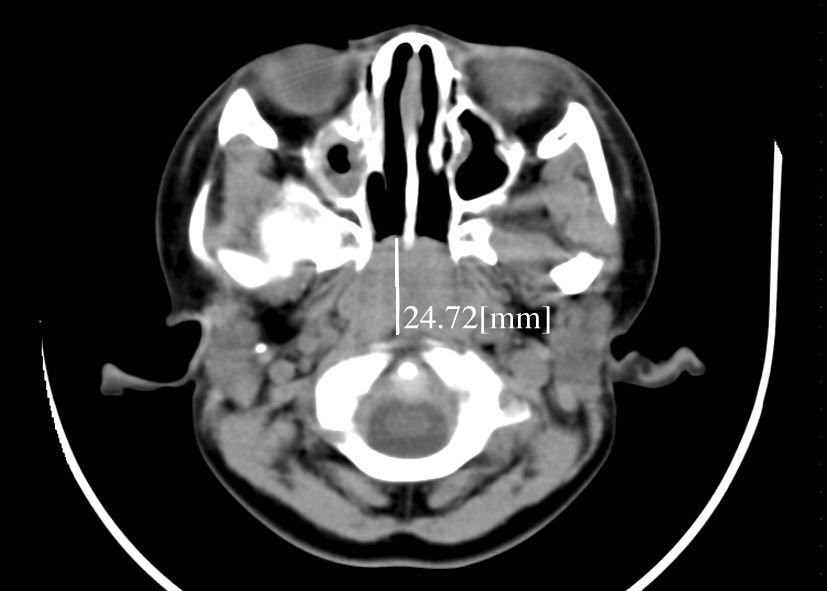
\includegraphics[width=.7\textwidth,height=\textheight,keepaspectratio]{./images/Image00142.jpg}
 \captionsetup{justification=centering}
 \caption{鼻咽腺样体肥大\\{\small 鼻咽顶壁和后壁软组织显著增生,密度均匀}}
 \label{fig6-5}
  \end{figure} 

鼻咽侧位片测量鼻咽顶部增殖腺的厚度和鼻咽腔的宽度,以两者比率来判断儿童增殖腺是否肥大。正常时两者比率≤0.60;当比率为0.61~0.70属中度肥大;比率≥0.71属病理性肥大。

\textbf{【鉴别诊断】}
主要与炎症鉴别,炎症表现为鼻咽部软组织较广泛的弥漫性肿胀,且伴有低密度分泌物。

\subsection{阻塞性睡眠呼吸暂停综合征}

本病亦称为阻塞性睡眠呼吸暂停低通气综合征(OSAHS),是指睡眠时上气道塌陷阻塞引起的呼吸暂停和通气不足,伴有打鼾、睡眠结构紊乱、血氧饱和度下降、白天嗜睡等临床表现综合征。本病多见于肥胖者。

\textbf{【病因病机】}
本病病因十分复杂,其直接发病机制是上气道的狭窄或阻塞、呼吸中枢的反应低下、中枢神经系统呼气时切断及吸气时接通机制的异常,其中70%由上气道阻塞引起。上气道狭窄的部位主要在软腭。严重者79%有软腭和舌根狭窄,中度者40%有上述异常。其原因为软腭变长而非增厚,由于软腭变长而成为钩状形态(约占9%)。软腭区是正常上气道最狭窄的部位,且肌肉对上气道的压力变化敏感。轻微的上气道的压力改变可触发软腭肌肉的活性,引起软腭长度的增加造成上气道狭窄。本病也可有多部位狭窄的特点,狭窄部位还包括下咽区、鼻咽等,尤以较严重者发生率高。另外有学者认为OSAHS患者睡眠过程中上气道易阻塞的原因,部分是由于这些部位本身存在结构上的狭窄,这些狭窄的原因可能为解剖结构异常、组织的水肿、肌张力的减弱、脂肪的沉积等,如扁桃体或增殖体(腺样体)肥大、鼻窦炎、鼻息肉、鼻中隔偏曲;上述的软腭增生肥大;舌根的淋巴组织增生及舌根后坠等。

\textbf{【临床表现】}
呼吸暂停的时间一般每次10秒以上,每夜发生5次以上。对本病的诊断,经典方法是采用多导睡眠图(PSG)监测,国际通用标准为每夜7小时睡眠过程中呼吸暂停及低通气反复发作30次以上,或睡眠呼吸暂停和低通气指数≥5。此外,本病易继发心血管疾病、神经系统疾病、白天易睡,应引起重视。

\textbf{【CT表现】}
应注意采用冠状和矢状面重建予以显示。冠状面尤其有利于显示扁桃体肥大,矢状面有利于显示悬雍垂-软腭及舌根部咽腔狭窄。OSAHS患者清醒时上气道的横断面积和各径线均小于正常人;睡眠时,由于颈部屈曲和上气道扩张肌的神经刺激减少,肌张力下降,吸气时上气道负压增加,使舌后的咽部塌陷,加重上气道的狭窄和阻塞。

\subsection{咽后及咽旁脓肿}

本病多见于3个月至3岁的儿童,约50%以上发生于1周岁内,这是由于儿童期咽后间隙中有多个淋巴结,在5岁后这些淋巴结逐渐萎缩。咽旁脓肿为咽旁间隙的化脓性炎症。

\textbf{【病因】}
以急性化脓性常见;慢性者多继发于结核,少数为梅毒和真菌所致。急性感染者常为上呼吸道感染后所致,其次为咽部尖锐性异物损伤后继发感染。

\textbf{【临床表现】}
患儿多先有上呼吸道感染史,并发热、畏寒、咽痛、吞咽困难,甚至有呼吸困难等症状。病程短,一般炎症经2~3天即可形成脓肿。结核性脓肿一般在1个月左右才形成。

\textbf{【CT表现】}
①由于咽后间隙左右有分隔,故初期可局限于一侧间隙,其内侧不超过中线。平扫鼻咽、口咽或喉咽部椎前或咽旁间隙软组织弥漫性肿胀伴脂肪间隙消失提示蜂窝组织炎。当组织坏死时,可见局限性低密度区,小低密度区融合成大腔即形成脓腔,如产气菌感染形成脓气腔。增强扫描脓腔壁强化。②结核性脓肿与化脓性脓肿表现相近,但可伴有钙化,脓肿壁多较厚,同时伴颈椎骨质破坏,易于同急性化脓性脓肿相鉴别(图\ref{fig6-6})。③急性咽后间隙炎症可并发环枢关节脱位或半脱位。



\begin{figure}[!htbp]
 \centering
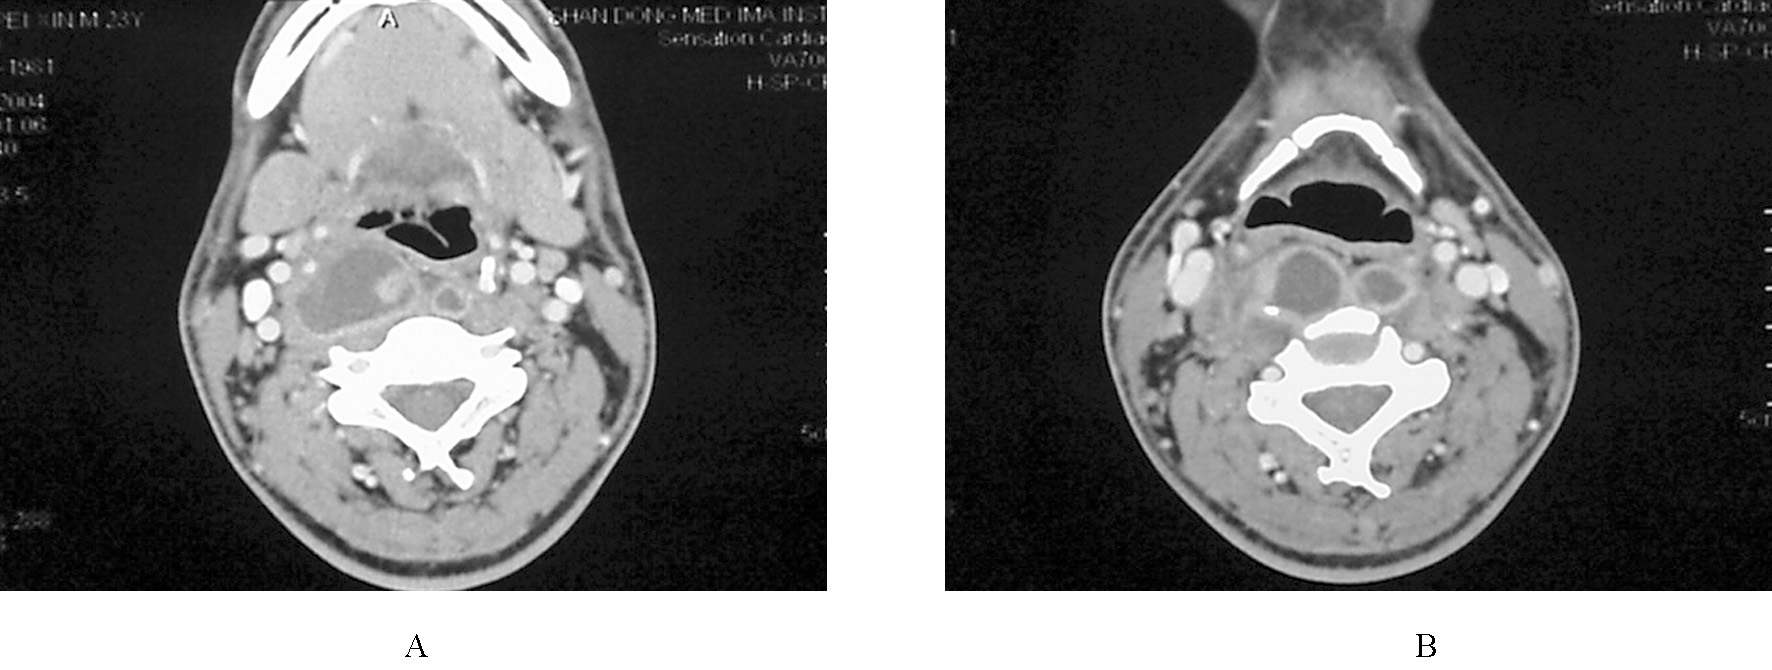
\includegraphics[width=.7\textwidth,height=\textheight,keepaspectratio]{./images/Image00143.jpg}
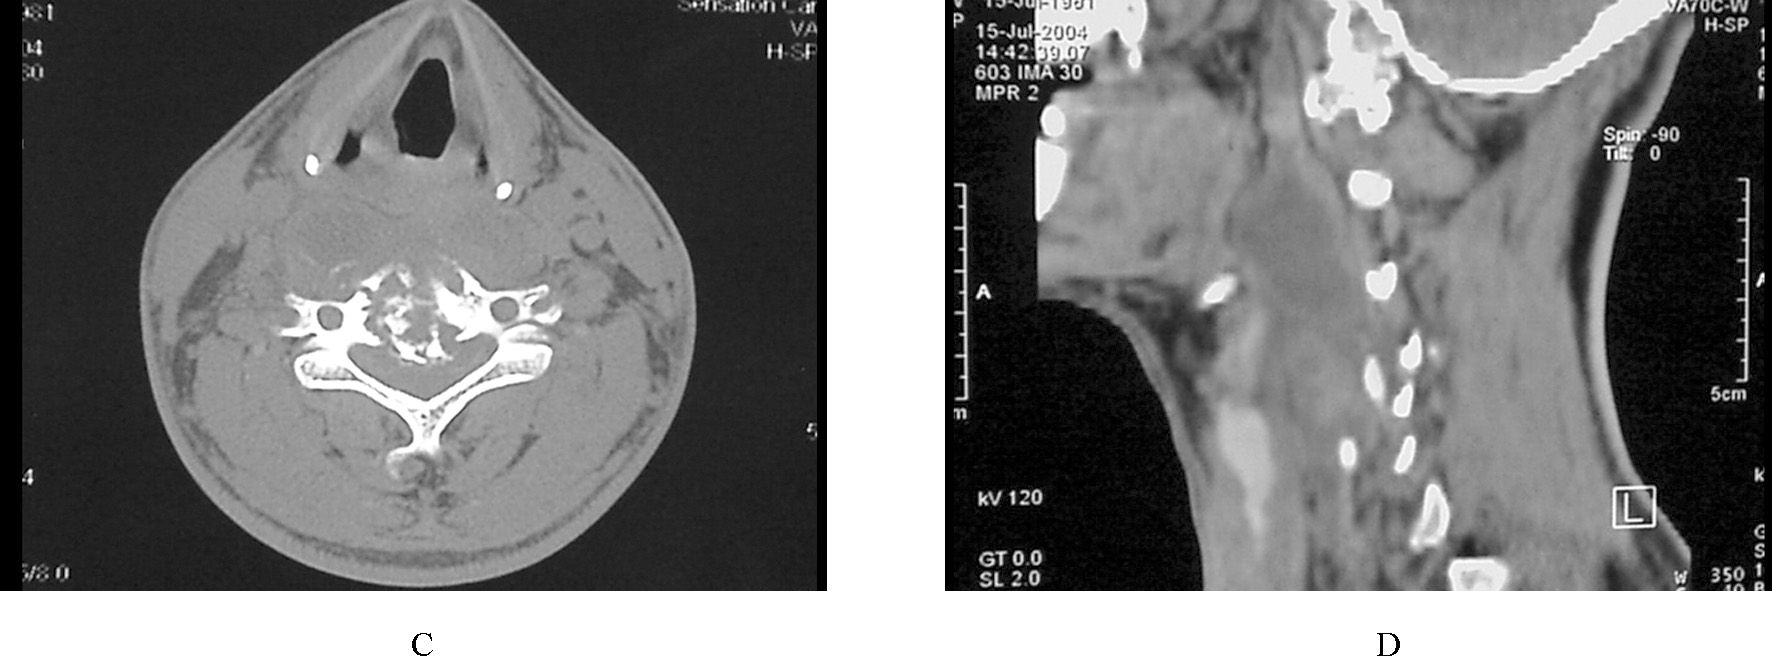
\includegraphics[width=.7\textwidth,height=\textheight,keepaspectratio]{./images/Image00144.jpg}
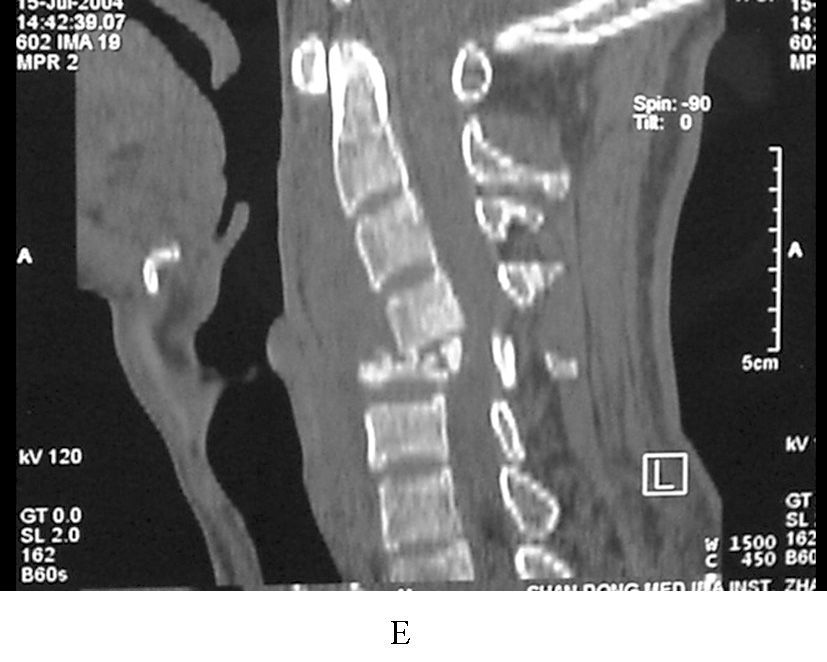
\includegraphics[width=.7\textwidth,height=\textheight,keepaspectratio]{./images/Image00145.jpg}
 \captionsetup{justification=centering}
 \caption{咽后结核性脓肿\\{\small A~E为同一患者,咽后间隙内有多个环状强化灶;C5椎体呈碎玻璃样骨质破坏,C4/5椎间隙变窄,C4后移位}}
 \label{fig6-6}
  \end{figure} 

\subsection{急性会厌炎}

本病为感染性疾病,起病急、发展快、来势凶为其特点。

\textbf{【病理】}
轻者会厌舌面黏膜充血肿胀或伴有杓会厌襞的肿胀,重者呈球形肿胀,甚至形成脓肿。

\textbf{【临床表现】}
可发生于任何年龄。咽喉疼痛、畏寒发热、吞咽困难和呼吸困难是最常见的症状。

\textbf{【CT表现】}
平扫可见会厌舌面、杓会厌襞增厚和会厌前间隙密度增高,界限不清,甚至杓状软骨区也有肿胀。脓肿形成早期可在低密度肿胀区内见密度较高的脓肿区,脓腔形成后呈低密度。成人一般不涉及声带以下;儿童因喉黏膜下组织较疏松,可有声门下区肿胀表现。

\subsection{慢性肥厚性喉炎及喉息肉}

本病是喉黏膜有较明显的增厚和过长,属细胞增生而非炎性肿胀。

\textbf{【病因病理】}
常因慢性喉炎患者不改变错误发音习惯和生活方式、工作环境所致。喉息肉是外伤性喉炎(歌手和职业上说话较多的人)的一种表现类型。病理表现为喉黏膜广泛增厚,以杓间区最为明显。声带充血,边缘圆厚、不平,可呈结节状或呈息肉状。室带也肥厚、粗糙不平,掩盖声带。杓状会厌襞也增厚。喉息肉多为纤维性或纤维血管性。

\textbf{【临床表现】}
有声音嘶哑、喉部不适及呼吸不畅等症状。喉镜可见喉黏膜充血、肿胀和声带息肉。

\textbf{【CT表现】}
①喉部结构肿胀增厚,以杓间区为著;室带、声带、杓会厌襞均增厚,声带不光整,两侧不对称。增厚黏膜强化不著。喉旁间隙和喉软骨均无异常。②喉息肉呈小的圆形结节,位于声带游离缘的前1/3与中1/3交界处,常为双侧,偶呈弥漫性生长。

\textbf{【鉴别诊断】}
①单纯慢性喉炎一般CT检查无明显异常,故多不需做CT检查。②喉部恶性肿瘤有喉旁间隙和喉软骨的浸润破坏是鉴别的关键。但有时需活检与肿瘤及其他炎症鉴别。

\subsection{喉结核}

本病多继发于肺结核,原发性非常少见。

\textbf{【感染途径】}
①直接接触感染:因带菌痰液易滞留于喉腔后部,故好发于后联合和杓间区;②血行、淋巴播散:病灶以会厌多见。因抗结核药物的应用,直接接触感染相对少见,目前以血行多见。

\textbf{【病理】}
分为3型:①浸润水肿型:多表现为喉黏膜弥漫性充血、会厌明显水肿、黏膜下有结核结节及小圆细胞浸润。②溃疡型:黏膜下结核结节向上发展,上皮破溃形成溃疡。多发生于会厌、声带及杓突部。病变发展可侵及软骨膜。③增生型:病变经长期治疗,部分呈瘢痕愈合,部分病灶形成结核瘤,均可导致喉狭窄。三者可同时存在、相互转化或以某种表现为主。

\textbf{【临床表现】}
本病好发于20~40岁,早期可无症状或仅干燥不适、灼热、干咳,进而咽痛、声音嘶哑等。此外,还可有肺结核的全身症状。

\textbf{【CT表现】}
根据病变的范围和病期可有两种主要表现:①弥漫型:多见于急性期,病变呈渗出性,软组织弥漫性肿胀增厚;②局灶型(肿块型):多为慢性期,病程较长,病变多以结节状肿块存在。

喉结核在影像学上:①大多表现为双侧弥漫性、不对称软组织肿胀增厚,涉及声带、室带、会厌和杓会厌皱襞,有强化;②可涉及或不涉及喉旁间隙和会厌前间隙,即使涉及也不出现喉腔外浸润性肿块;③喉的支架都保持完整,多无喉软骨增生硬化和骨质破坏;④喉结核虽可涉及咽部、扁桃体和软腭,但较少涉及喉咽和声门下区;⑤慢性期可有局灶性肿块、瘢痕粘连、喉狭窄等表现;⑥半数患者伴有颈部淋巴结结核。

\textbf{【鉴别诊断】}

1.喉癌:①喉癌有不规则的软组织肿块增生,可有相对清楚的边缘,可向会厌前间隙和喉旁间隙浸润;而喉结核两侧弥漫不对称肿胀,喉旁间隙及会厌前间隙可不受侵(尤其慢性期多无受侵。)②喉癌可破坏喉部软骨,喉的支架有变形;而结核则无。③喉癌可出现喉外肿块;而结核多不会。④喉癌可侵及喉咽及声门下区;而结核则很少。但老年患者的肿块型喉结核常需组织学确诊。

2.急、慢性喉炎:①结合临床、局部症状和肺部表现与急性喉炎多可鉴别。②与慢性肥厚性炎症不易鉴别。一般慢性喉炎可表现为喉黏膜不均匀性普遍增厚,杓会厌皱襞、杓状软骨、室带及声带不对称肥厚,边缘不整,多无特异性。慢性炎症与其他疾病的鉴别需借助于活检。

3.喉淀粉样变性:①弥漫浸润型:见声门上下气道前壁、后壁局部增厚,部分可有斑点状钙化。②结节型:在室带、喉室、声带处见类似于乳头状瘤样改变,多伴有深部浸润,但不破坏喉软骨。影像学表现很难与局灶型喉结核和喉癌鉴别。

\subsection{喉白喉}

喉白喉较咽白喉少见。有时可单独发生,且可向气管内蔓延,窒息情况多较严重。

\textbf{【影像学表现】}
急性期由于假膜附着于声带附近,喉内结构显影模糊不清。白喉后遗狭窄则很少见,表现为喉及声门下气道变小。总之,本病并无特异性影像学表现。

\subsection{喉梅毒}

喉梅毒极少见,就诊病人多属晚期病变。

\textbf{【影像学表现】}
增殖性炎症影像学表现为喉部软组织肿胀增厚,表面高低不平为溃烂表现,常导致部分结构缺损,以会厌为著。软骨炎症可导致骨质疏松破坏。晚期多有粘连变形及喉腔狭窄。总之,影像学表现无特异性,主要依靠临床及实验室检查诊断。

\subsection{喉淀粉样变性}

本病少见,且影像学表现与喉肿物很难鉴别。

\textbf{【病因病理】}
尚未完全阐明,主要有两种观点:①淀粉样变性与机体蛋白代谢失调有关。由于全身蛋白代谢障碍,致淀粉样物在全身各器官沉积。②局部淀粉样变性是由于某种原因形成局部代谢障碍,致淀粉样物沉积于局部的结果;也有人认为局部淀粉样变性是当某一器官慢性炎症时,血液循环和淋巴循环发生阻滞,局部蛋白代谢紊乱和球蛋白沉积所致;亦有人认为局部的慢性炎症可能为主要原因,是局部组织的长期慢性炎症而引起的一种自身免疫过程。

按其病理形态分为局限肿块型和弥漫浸润型两类,后者多为呼吸道或全身淀粉样变性的表现之一。

\textbf{【临床表现】}
多见于40~70岁,男性略多。无特征性表现,常见喘鸣、声音嘶哑、呼吸和吞咽困难等。

\textbf{【CT表现】}
①局限肿块型:或称结节型。病变多侵及喉前庭、室带和声门下区。可见单个或多个大小不一(可达2.0~3.0cm)的结节状隆起,表面光整,密度均匀。可伴深部浸润,但不破坏喉软骨。②弥漫浸润型:病变广泛侵及双侧或单侧喉前庭、室带及声门下区,以弥漫肥厚和水肿为主要表现。本病可出现不同程度的钙化,晚期可发生喉、气管纤维化狭窄。

总之,本病有以下特点:①病程较长,临床以反复发作性声音嘶哑,且时轻时重为其特点之一;②影像学表现多以喉部肿块为主要表现,且病变范围多较广泛,部分可发生钙化,密度较常见的肿瘤高;③仅靠影像学难以与喉癌鉴别。

\section{肿瘤}

\subsection{概述}

\subsubsection{咽、喉部良性肿瘤}

1.咽部良性肿瘤:种类较多,但发生率不高。①鼻咽纤维血管瘤是鼻咽部最常见的良性肿瘤,此外,还可见神经源性肿瘤、囊肿、颅咽管瘤等。②口咽部良性肿瘤较恶性肿瘤明显少见,其中甲状舌管囊肿并不少见(青少年多见);真正的良性肿瘤则很少见,如神经源性肿瘤、混合瘤、错构瘤等。③喉咽部(下咽部)肿瘤来自中胚层或上皮。良性肿瘤极少见,常见的为纤维脂肪瘤和平滑肌瘤,其他少见的为小唾液腺瘤、腺瘤、囊腺瘤。

2.喉部良性肿瘤:很少见,能见到的有乳头状瘤,可发生于气道的任何部位,诊断主要依靠喉镜;其他少见的良性肿瘤有软骨瘤、血管瘤和神经纤维瘤。软骨瘤多起源于环状软骨的后骨板;神经纤维瘤见于杓会厌皱襞和室带水平;血管瘤发生部位不定。

\subsubsection{咽、喉部恶性肿瘤}

1.咽部恶性肿瘤:发生率较高。①鼻咽部恶性肿瘤以鼻咽癌最常见,非霍奇金病占第二位;在儿童中以横纹肌肉瘤最常见。颈部神经母细胞瘤也可见于鼻咽部,其他少见的肿瘤还有颅底脊索瘤、软骨肉瘤、纤维肉瘤或骨肉瘤。黑色素瘤、嗅神经母细胞瘤原发于鼻腔,但可累及鼻咽部。浆细胞瘤、颅底转移瘤、咽后淋巴结转移瘤亦可表现为鼻咽部肿物。②口咽部黏膜源性肿瘤最为多见,98%为癌。口咽部淋巴组织丰富,故淋巴瘤亦很常见,它与鼻咽淋巴瘤是最常见的头颈部结外NHL的发病部位。③下咽部恶性肿瘤多半为鳞癌,以梨状窝为常见部位。

2.喉部恶性肿瘤:以鳞癌最多见,约占95%,其次为喉乳头状瘤恶变,而未分化癌、淋巴肉瘤和腺癌等少见。

\subsubsection{颞下窝、翼腭窝的肿瘤}

主要来源于邻近肿瘤的侵犯,例如上颌窦癌、鼻咽癌以及部分良性肿瘤等。咽部、下颌部位的原发性肿瘤亦可侵及颞下窝。血源性肿瘤往往先至下颌骨,而后向颞下窝蔓延。

颞下窝、翼腭窝内的原发性肿瘤多为肉瘤或未分化癌,如淋巴瘤、上颌窦骨肉瘤、神经纤维肉瘤、血管肉瘤、横纹肌肉瘤等。亦可见腺样囊性癌、腺癌、鳞癌、恶性纤维组织细胞瘤等。但涎腺肿瘤多不发生于颞下窝内。良性肿瘤有咬肌血管瘤、下颌骨良性肿瘤,以及咀嚼肌间隙内的脂肪瘤、血管平滑肌瘤、神经源性肿瘤及牙源性含齿囊肿。

\subsection{鼻咽纤维血管瘤}

本病又称青年鼻咽血管纤维瘤、男性青春期出血性纤维瘤等,是鼻咽部最常见的良性肿瘤。

\textbf{【病理】}
该瘤起源于蝶骨体、枕骨基部及鼻后孔,有报道亦可起源于蝶腭孔。多呈类圆形、结节状或分叶状。其主要成分为纤维组织和血管组织,无包膜。

\textbf{【临床表现】}
好发于10~25岁的男性青少年,偶见于儿童。鼻塞和鼻出血为两个基本症状。阻塞咽鼓管、鼻旁窦口或侵及鼻旁窦、眼眶等出现相应症状和体征。国内有学者将其分为4个临床类型:①鼻咽鼻腔型;②鼻咽软腭型;③鼻咽翼颊型;④鼻咽颅眶型。

\textbf{【CT表现】}
应注意观察肿瘤的涉及范围和与周围大血管的关系。瘤体与肌肉密度相仿,故平扫其界限不清。增强扫描瘤体明显强化,其CT值升高40Hu以上,可超过100Hu;瘤体呈椭圆形或分叶状均质高密度肿块,边缘清晰。瘤体内一般不含钙化灶和静脉石。周围组织有压迫性改变如骨受压变形、肌组织或间隙向外移位。冠扫有助于了解肿瘤侵入眼眶、筛窦、蝶窦、海绵窦和颅中窝的情况。

\textbf{【鉴别诊断】}
①鼻腔及鼻后孔息肉:较鼻咽纤维血管瘤密度低且无明显强化可以鉴别。②鼻咽癌:呈浸润性生长,边缘不清,强化不如鼻咽纤维血管瘤显著,常伴颅骨溶骨性破坏可予鉴别。③增殖体肥大:临床上与鼻咽纤维血管瘤不难鉴别;增殖体肥大密度和强化较鼻咽纤维血管瘤低可以鉴别。

\subsection{咽部神经源性肿瘤}

咽部良性神经源性肿瘤的命名过去不甚统一。目前将其分为神经鞘瘤和神经纤维瘤两类。多发生于外周颅神经、交感神经及其分支,好发于咽后壁及其侧壁。

\textbf{【临床表现】}
早期较小时无症状。大者可有咽部不适或异物感,甚至出现吞咽困难。肿瘤压迫喉和气管时可有语言改变和呼吸困难。涉及后组脑神经可引起第Ⅸ、Ⅹ、Ⅺ、Ⅻ脑神经症状。

\textbf{【CT表现】}
多位于咽部间隙内,也可发生于咽后壁,上起鼻咽顶部,下至喉咽平面的任何部位。肿瘤多呈类圆形,界限较清。平扫时与肌组织密度相近或略低,神经纤维瘤较神经鞘瘤密度高;肿瘤有低密度囊变区是神经鞘瘤的特征。增强扫描轻度强化。因肿瘤起源于颈动脉鞘内的第Ⅸ、Ⅹ、Ⅺ、Ⅻ颅神经和交感神经链,故肿瘤常将咽旁间隙及颈内动脉向外后推移,有助于同咽黏膜间隙和腮腺间隙的占位鉴别。

\textbf{【鉴别诊断】}
咽部血管源性肿瘤显著强化有助于鉴别。扁桃体恶性肿瘤可向咽侧壁深部浸润,并将咽旁间隙向后推挤有助于鉴别。腮腺间隙的占位常将咽旁间隙及颈内动脉向后内推移有助于鉴别。

\subsection{喉乳头状瘤}

本病是一种起源于上皮组织的良性肿瘤。单发者多见于成人,偶发于儿童。而多发者主要见于10岁以下儿童,并在术后极易复发。

\textbf{【病因病理】}
病因有以下学说:病毒感染、慢性炎症刺激和内分泌学说,目前大多支持病毒感染学说。其主要病理改变为复层鳞状上皮及其下的结缔组织向表面呈乳头状增生,富含血管。在儿童时期很少恶变,而成人易恶变。

\textbf{【临床表现】}
成人以声音嘶哑为主要症状,儿童早期为声音嘶哑或异常哭声,以后出现喘鸣及急性呼吸困难。

\textbf{【CT表现】}
小的病变可无阳性发现。单发病变可见声带、室带、前联合或声门下区不光整、增厚呈团块状,病变可有明显钙化。增强扫描明显强化。一般不向深部浸润,如成人有深部浸润应考虑恶变可能。多发者可表现为彼此分散的肿块,或融合成大块状,表面呈菜花状或分叶状,但均无深部浸润改变。

\subsection{舌癌}

本病临床易于确诊,CT检查较少应用。

舌的正常CT表现:以舌中隔、正中线、正中缝为中线,双侧结构对称。加以斜、纵行条带状低密度区,为舌肌间脂肪组织且其位置、大小均较对称。由于舌本身的CT表现就可见到低密度区,因此首先应注意其正常表现,以免把正常误为病变。其次应注意双侧低密度区是否对称、大小是否相近。若一侧的低密度区较小或较大均提示有病变存在,此时增强扫描可明确显示病灶。

\textbf{【舌癌的CT表现】}
①溃疡型:平扫多为低密度,导致一侧低密度区的增大;②疣型:平扫多为等或略高密度区,导致一侧低密度区变小;③增强扫描:肿瘤实质部分轻至中度强化,坏死区不强化,故呈环形强化或不均匀强化。

总之,舌癌的诊断平扫时应注意舌双侧结构的对称性,并应平扫加增强以更好的显示病灶。

\subsection{鼻咽癌}

本病是我国最常见的鼻咽部恶性肿瘤。我国是高发区,南方沿海地区居民发病率明显高于北方和内地,尤以珠江三角洲地区发病率最高。

\textbf{【病因病理】}
其病因不甚明确,但与慢性炎症、遗传和EB病毒感染有关。

按组织学分类:本病为鼻咽黏膜上皮发生的癌肿,90%以上为鳞癌,少见的有泡状核细胞癌、腺癌、未分化癌等。

按肿瘤原发部位形态可呈:①结节型;②菜花型;③黏膜下型;④浸润型;⑤溃疡型。以结节型最常见,溃疡型少见。黏膜下型常以颈部淋巴结肿大或远处转移为初发症状就诊。鼻咽癌可多中心生长。

按分化程度分为:①未分化癌:占54.5%;②低分化癌:占30.8%,大多是Ⅲ~Ⅳ级鳞癌;③较高分化癌:占11%,为Ⅰ~Ⅱ级鳞癌和腺癌。

按发展方向分为:①上行型:又称为颅神经侵犯型。破坏颅底骨,常侵犯Ⅲ~Ⅵ颅神经即前组颅神经,经颈淋巴结转移少见。②下行型:又称颈部肿块型。常见颈淋巴结肿大,一般无颅底骨破坏,可有第Ⅸ~Ⅻ颅神经即后组颅神经受损。③混合型。其中上行型和下行型以低分化癌多见,混合型以未分化癌多见。

\textbf{【转移途径】} ①
直接扩散:破坏中后颅窝底部,侵入蝶窦、海绵窦而涉及Ⅲ~Ⅵ颅神经,向后破坏颈静脉孔可涉及Ⅸ~Ⅻ颅神经。极少穿破硬脑膜侵犯脑实质。②淋巴转移:最早转移至咽后侧组淋巴结、颈深上组和颈后三角区副神经淋巴结,以后可到其他深组淋巴结。双侧转移者也很常见。第Ⅸ~Ⅻ颅神经和颈交感神经节亦可因肿大淋巴结压迫而受累。③远处转移:通过血行可转移至肺、肝、骨等部位。

\textbf{【临床表现】}
可发生于任何年龄,国内统计可发病于3~86岁,以40~44岁发病最多,70岁以后逐渐下降。男性明显多于女性,其比率为2~10∶1。初发症状按顺序排列如下:回缩涕带血、鼻塞、颈部淋巴结增大、听力下降、耳鸣、头痛和复视等。进而侵犯海绵窦之Ⅲ、Ⅳ、Ⅵ颅神经出现海绵窦综合征(复视、眼肌麻痹症状)和颈静脉窝综合征(第Ⅸ~Ⅻ颅神经受损害的表现),以及颅底神经受损的表现。鼻咽镜检查肿瘤呈紫红色,触之易出血。约50%以上病例可有渗出性中耳炎的鼓室积液。

\textbf{【CT表现】} 最常见于鼻咽顶部,其次为侧壁,前壁和底壁极少。

1.平扫表现:①咽隐窝是最常见的原发部位,故一般表现为咽隐窝变浅或消失,咽腔两侧不对称(图\ref{fig6-7}A、B)。②另一重要表现是咽肌的增厚和不对称,主要为腭肌的浸润和肥大(最先表现为腭帆提肌肥大)。③咽鼓管阻塞表现为中耳和乳突蜂窝气体消失即渗出性中耳炎之征象。④咽旁间隙外移也是一个较有特征的表现。⑤鼻咽癌向后可直接累及椎前肌肉并可致淋巴结肿大,向下致软腭增厚。向颅内蔓延常常是经破裂孔至海绵窦,眶尖可受累;另一常见途径是经卵圆孔向颅内蔓延,引起卵圆孔扩大(临床表现咀嚼肌萎缩)。也可直接侵犯颞下窝引起肌肉肿大、肌间隙消失(张口困难)。⑥颈淋巴结肿大。

2.增强扫描:平扫肿瘤密度稍低于肌肉,但高于脑组织,界限不清,形态不规则。增强扫描肿瘤强化较著,CT值升高20Hu以上,使肿瘤界限更清晰;并有利于显示咽旁间隙、颈动脉鞘、海绵窦受侵情况。

3.颅底骨破坏的CT表现分为3类:①成骨型:骨外形无明显变化,可能是肿瘤压迫产生缺血、硬化增生或者是对肿瘤的反应性增生所致,还有人认为硬化是破坏的初始阶段(图\ref{fig6-7}C);②溶骨型(图\ref{fig6-7}D);③混合型。颅底骨破坏均与原发病灶位于同侧,且多伴有同侧头痛。此外,病灶可经破坏的颅底直接侵及脑内(图\ref{fig6-7}E)。



\begin{figure}[!htbp]
 \centering
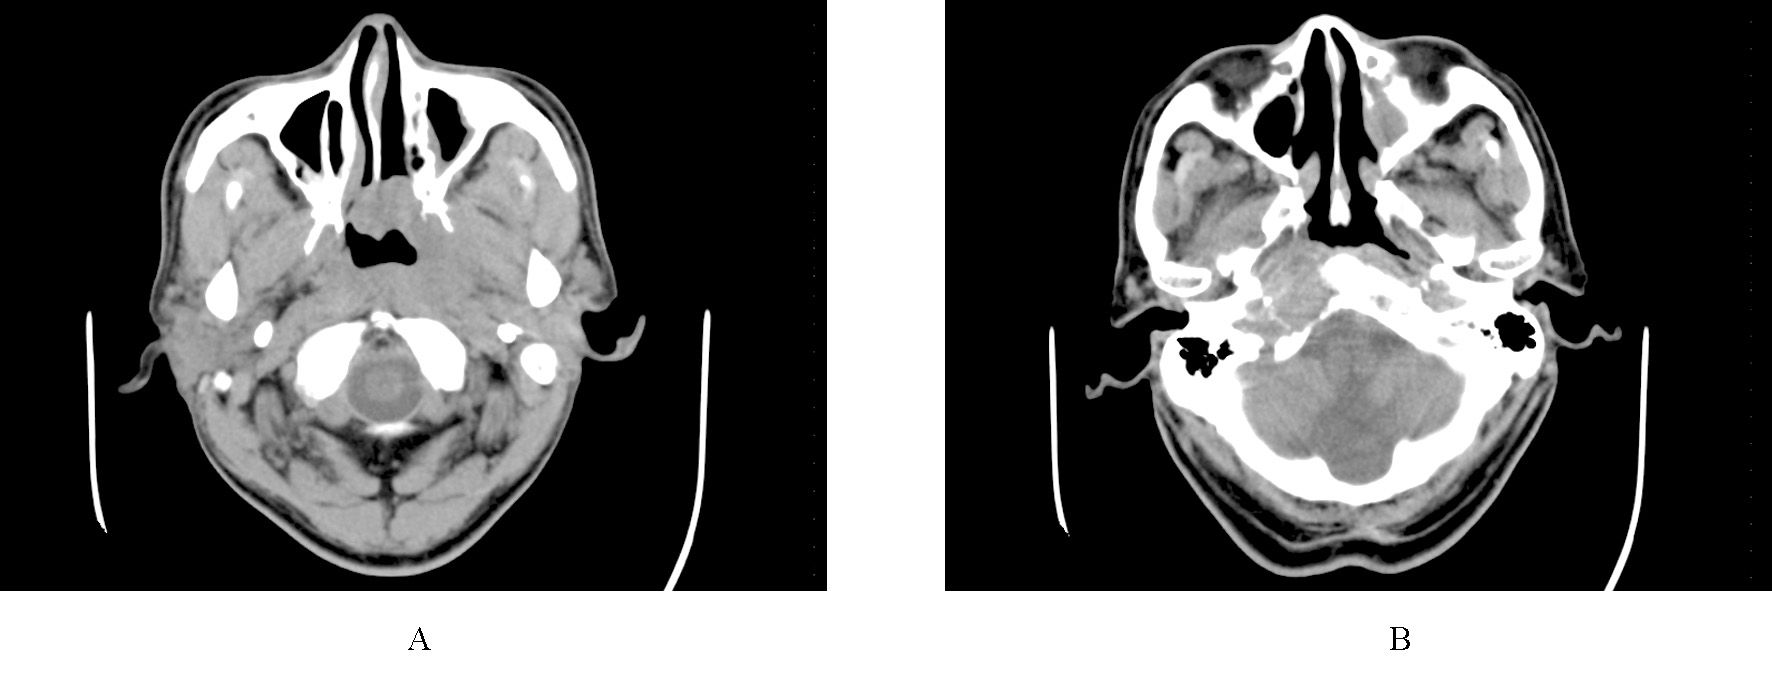
\includegraphics[width=.7\textwidth,height=\textheight,keepaspectratio]{./images/Image00146.jpg}
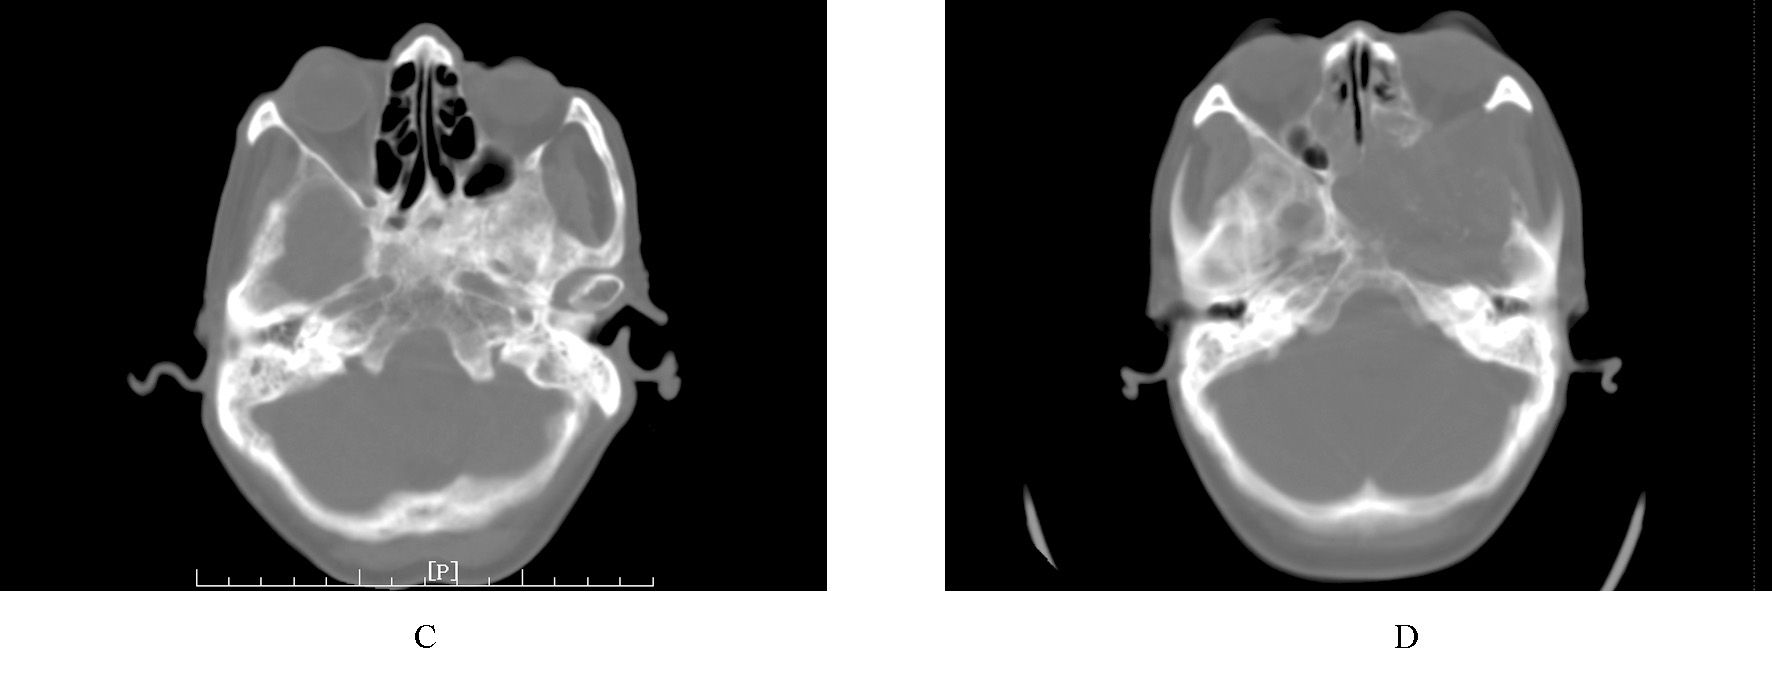
\includegraphics[width=.7\textwidth,height=\textheight,keepaspectratio]{./images/Image00147.jpg}
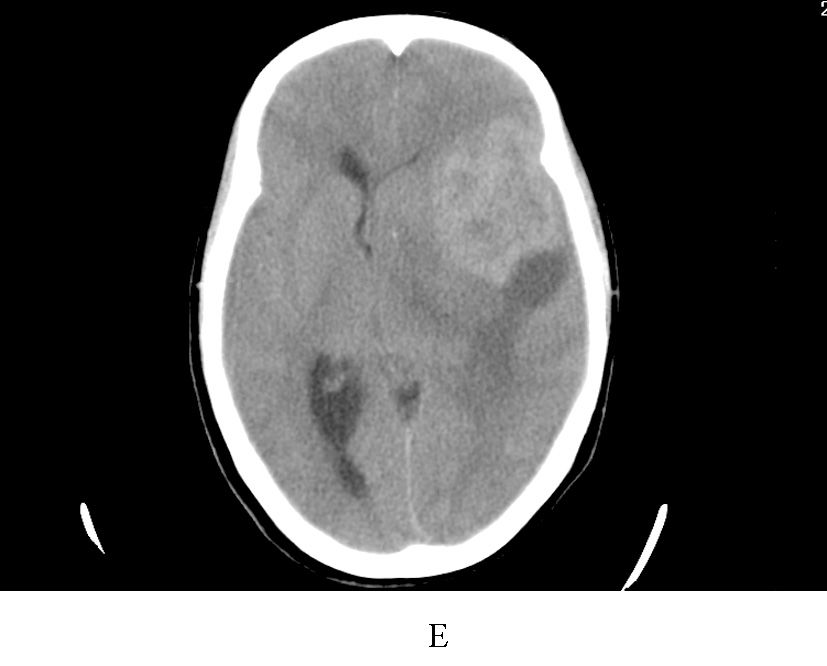
\includegraphics[width=.7\textwidth,height=\textheight,keepaspectratio]{./images/Image00148.jpg}
 \captionsetup{justification=centering}
 \caption{鼻咽癌\\{\small A.病灶主要位于鼻咽顶壁和左侧壁,并涉及后鼻孔区;双侧咽隐窝消失,左侧咽旁间隙受侵;B.病灶主要位于鼻咽右侧壁,右侧咽隐窝消失,颅底右侧骨质破坏;C.鼻咽癌致颅底骨质硬化;D.鼻咽癌致颅底左侧溶骨性骨质破坏;E.鼻咽癌浸入左侧大脑半球}}
 \label{fig6-7}
  \end{figure} 

4.咽旁间隙受侵的判断:国外有学者取内侧翼板游离缘与颈内动脉外缘的连线为第一线;内侧翼板基底部舟状窝与茎突连线为第二线;外侧翼板的游离缘与下颌升支后缘的连线为第三线。肿瘤浸润范围未达第一线为无咽旁间隙浸润,达到或超过第一线为Ⅰ型浸润,依次称为Ⅱ、Ⅲ型浸润。

\textbf{【鉴别诊断】}

1.鼻咽部淋巴组织残留或增生:10岁以后退化,个别成人仍有较大增殖体存在。淋巴腺样体的增生表现为顶后壁软组织的对称性增厚或小丘状隆起,但椎前肌肉轮廓间隙或咽缝应能清楚显示、咽旁间隙无侵犯。此外,慢性炎症多表现为后壁或顶后壁软组织弥漫性对称性增厚,亦无上述间隙侵犯,应注意鉴别。

2.鼻咽纤维血管瘤:多见于20岁左右青年男性,持续鼻塞和反复出血。无论平扫和增强CT值均高于鼻咽癌,且强化较鼻咽癌显著。邻近骨质压迫性吸收破坏。

3.鼻咽部结核:较喉结核少见。CT表现密度不均、边界不规则或与邻近组织之间有条索状的粘连,骨质大片状破坏、硬化甚至死骨形成。孤立的死骨是结核的特征。颈部有串珠状多发较小淋巴结增大,甚至伴有钙化与鼻咽癌有别。

4.脊索瘤:颅底中线部较广泛的溶骨性、膨胀性骨质破坏,伴有软组肿块,其内多有残存碎骨片及钙化表现。无明显强化。

5.淋巴瘤:为全身淋巴瘤的局部表现,亦可孤立生长于鼻咽部。除鼻咽部肿块外,咽后、两侧咽旁可同时有肿块形成并融合,边缘凹凸不平,以及颈部、其他部位淋巴结广泛增大。

6.蝶窦恶性肿瘤:肿块大部位于蝶窦,窦壁骨质破坏,蝶窦扩大。冠状位有助于鉴别。

7.恶性肉芽肿:可见鼻咽部较大肿块,有时累及鼻腔,可同时向两侧咽旁及咽后间隙侵犯,少有颈部淋巴结增大。但常鉴别困难。

8.结节病:国内有学者报道1例类似鼻咽癌的结节病,但咽旁间隙不受侵,结合胸部改变可予鉴别。

9.鼻咽癌放疗后复发与纤维化鉴别:放疗后局部复发与纤维化多表现为软组织肿块,两者在CT平扫和常规增强扫描上密度比较接近而极难鉴别。国内有学者以2.5ml/s流率、对比剂用量1ml/kg体重进行动态增强扫描,发现各有以下特点:①放疗后纤维化:是由于放疗致使肿瘤组织变性坏死,由增生的结缔组织替代而成。由于血供差故增强扫描程度多较弱且上升缓慢,增强后200秒以前其CT值多呈缓慢上升,至200秒左右达峰值,其后缓慢下降。即动态增强的时间-密度曲线呈缓升-缓降型。②放疗后复发肿块:由于血供丰富,故动态增强CT值迅速上升,约在120秒左右达到峰值,其后呈缓慢下降。其时间-密度曲线呈速升-缓降型,且复发肿块的CT值显著高于纤维化者。

\subsection{口咽癌}

\textbf{【病理】}
口咽癌主要包括舌后1/3的舌根部癌、扁桃体癌、软腭癌、口咽侧壁癌(包括舌腭弓癌和咽腭弓癌),其中90%~95%为鳞癌,还有腺样囊性癌、腺泡细胞癌、黏液表皮样癌、未分化癌、基底样癌、梭状细胞癌等。由于其位置深在、侵袭性强,早期就有淋巴结转移。

\textbf{【临床表现】}
以中老年多见,男性多于女性。主要表现为咽部不适、异物感,咽痛,吞咽受阻,可发现咽部肿块或无意中发现颈部肿块。

\textbf{【CT表现】}
病变多位于一侧,肿块形态不规则,界限不清,易侵犯邻近结构。因肿瘤血供丰富,增强后多有不同程度的强化,其内部密度多不均匀。咽旁间隙狭小、外移或受侵;亦可侵及舌下间隙。常可发现颈部转移增大的淋巴结。

\textbf{【鉴别诊断】}
主要应与淋巴瘤相鉴别,有以下不同:①口咽癌多为单侧病变;而淋巴瘤常侵犯双侧扁桃体。②两者形态多不规则,但口咽癌常侵犯周围结构,边缘多不清楚;淋巴瘤少有深部侵犯,边界常清楚。③口咽癌血供丰富,增强后多有不同程度的强化,且内部密度多不均匀;淋巴瘤强化多不明显,且密度均匀。④淋巴瘤颈部淋巴结受侵相当常见,在头颈部恶性肿瘤中仅次于鳞癌转移,两者难以鉴别。但淋巴瘤颈部淋巴结受侵多为双侧多发,边界规则,密度相对均匀,等于或略高于肌肉密度,其内可见小低密度区,少部分可见与转移鳞癌相似的边缘环形强化。颈后三角区及浅表淋巴结受累亦更多见于淋巴瘤。

此外,国内有学者认为:多部位多中心起源、大肿块或咽壁弥漫浸润性增厚、颅底及深层侵犯少是咽淋巴环非霍奇金淋巴瘤的典型影像学表现。

\subsection{扁桃体恶性肿瘤}

本病是口咽部最常见的肿瘤。

\textbf{【病理】}
大致分为鳞癌、淋巴上皮癌和淋巴肉瘤,此外还有未分化癌和各种类型的淋巴瘤。约60%有颈部淋巴结转移,约20%转移至对侧颈部淋巴结;晚期约10%~20%有远处转移。

\textbf{【临床表现】}
癌肿好发于50~60岁,肉瘤发病年龄较轻,男性多于女性。早期症状不明显,仅有咽部不适、异物感,体检可见一侧扁桃体肿大、质硬、可有溃疡。晚期咽部明显疼痛,并可向邻近耳部、面部放射。

\textbf{【CT表现】}
可见一侧口咽侧壁软组织增厚,癌肿向周围浸润,边界不清,表面饱满;咽旁间隙狭小、外移。如为淋巴瘤多呈巨块型,可见有肿块突入口腔内。增强扫描可有轻至中度强化,并有利于显示其浸润范围及有无颈部淋巴结转移。

\subsection{咽淋巴环淋巴瘤}

咽淋巴环包括鼻咽、软腭、扁桃体、口咽以及舌根在内的环状淋巴组织,国内是非何杰金淋巴瘤(NHL)常见的结外侵犯部位,占全部NHL的19%;而在美国最常见的部位是胃肠道,咽淋巴环次之,约占全部NHL的5%~10%。

\textbf{【病理】}
欧美等国咽淋巴环NHL主要为B细胞来源,T和NK/T细胞来源少见,而在我国T和NK/T细胞来源发病率较高。可分为肿块型、浸润型、溃疡型和混合型。

\textbf{【临床表现】}
国内报道1组,年龄8~81岁,中位年龄50岁。可有咽部不适及咽痛、涕血及鼻塞、颈部肿块、头痛、面部麻木、复视、声音嘶哑,还可有发热、盗汗及体重下降等。

\textbf{【CT表现】}
一般认为无特异性。有学者根据CT和MR大致分为肿块型、浸润型、溃疡型和混合型。以肿块型最多见,其次为浸润型。可多部位、多中心起源。肿块型以突向腔内生长为主,界限清晰、边缘光整,密度均匀;浸润型病变较弥漫,常表现为整个咽淋巴环乃至下咽部弥漫性、对称性环状增厚,界限不清,部分密度不均;单纯溃疡型较少见,CT不易显示(MR可见黏膜线中断)。各型病变均以局限于咽黏膜间隙内多见,咽旁等深部间隙以受压外移或变窄为主,受侵少见。颅底骨质破坏也少见。此外,常可见双侧颈部淋巴结肿大。

总之,多部位多中心起源、大肿块或咽壁弥漫浸润性增厚、颅底及深层侵犯少是咽淋巴环NHL的典型影像学表现(图\ref{fig6-8})。



\begin{figure}[!htbp]
 \centering
 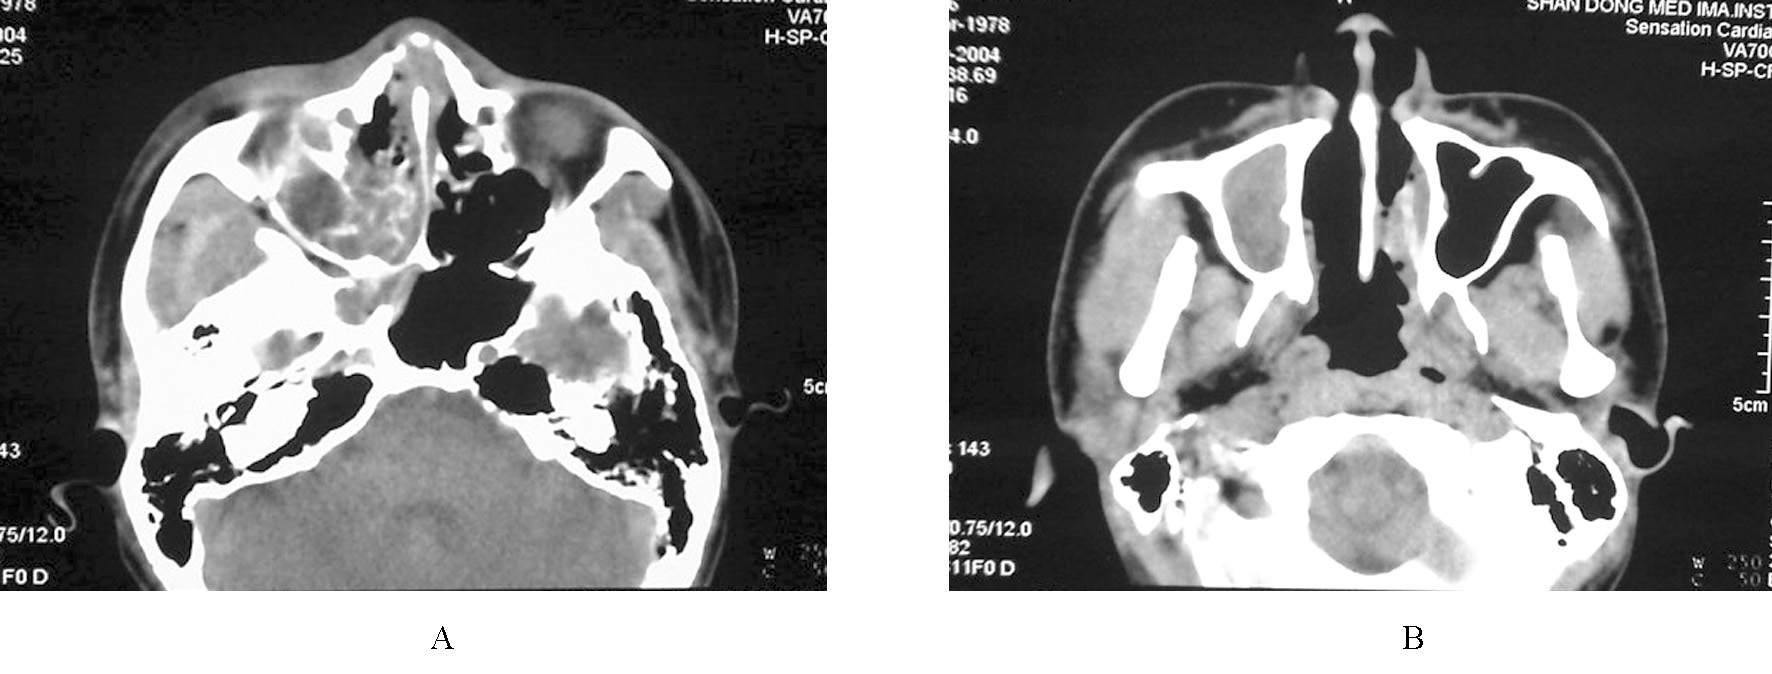
\includegraphics[width=.7\textwidth,height=\textheight,keepaspectratio]{./images/Image00149.jpg}
 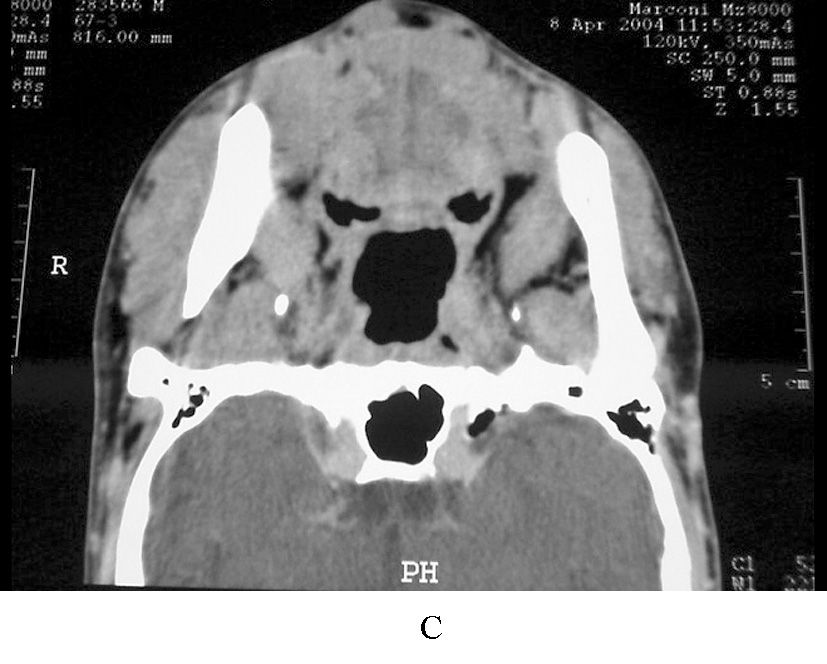
\includegraphics[width=.7\textwidth,height=\textheight,keepaspectratio]{./images/Image00150.jpg}
 \captionsetup{justification=centering}
 \caption{鼻腔、鼻咽部淋巴瘤\\{\small A~C为同一患者。双侧鼻腔前部、右侧鼻腔有软组织密度灶;右侧上颌窦、筛窦、蝶窦密实;右侧鼻咽部软组织增厚、咽鼓管隆突增大}}
 \label{fig6-8}
  \end{figure} 

\subsection{下咽癌}

本病亦称喉咽癌,较少见,在我国其发病率远低于喉癌。

\textbf{【病因病理】}
其病因不明,可能与咽部和口腔的慢性炎症、长期烟酒刺激有关。临床上将其分为梨状窝癌(70%~86%)、下咽上区癌(位于会厌舌面及会厌前间隙,占9%)、环状软骨后癌(环后区癌,占5%)和咽后型癌(下咽后壁癌,占5%~22%),肿块较大时不易区分。多半为鳞状细胞癌,淋巴结转移率高达60%~70%。

\textbf{【临床表现】}
好发于40岁以上的中老年人。早期症状不著,吞咽时一侧咽喉不适或轻微吞咽痛为主要症状。晚期有吞咽困难、声音嘶哑、顽固性一侧喉咽疼痛或伴同侧耳部放射痛。60%以上有淋巴结转移,甚至为最早表现。

\textbf{【CT表现】}
钡剂梨状窝食管造影X线检查优于CT。CT表现为:①一侧杓会厌皱襞增厚,梨状窝呈环形狭小甚至闭塞(图\ref{fig6-9})。②肿瘤向外侧可破坏甲状软骨或舌骨;向后内可使咽后壁软组织增厚;超过中线可侵及对侧咽后壁及食管入口周围;向前内侵及会厌、会厌前间隙、破坏甲状软骨,经声门旁间隙进入喉腔。③瘤内无钙化、囊变或坏死等改变。④增强扫描稍有强化或肿瘤界限显示较清晰。⑤国内有人测定杓-椎距(杓状软骨至颈椎前缘间距)或环-椎距(环状软骨至颈椎前缘间距),>1cm对下咽癌诊断有价值。

\begin{figure}[!htbp]
 \centering
 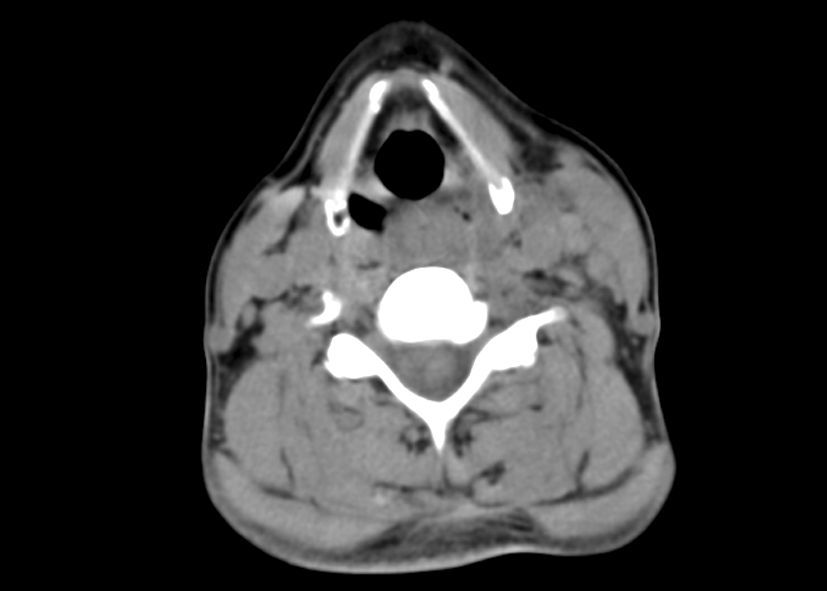
\includegraphics[width=.7\textwidth,height=\textheight,keepaspectratio]{./images/Image00151.jpg}
 \captionsetup{justification=centering}
 \caption{下咽癌\\{\small 咽后有软组织肿块,左侧梨状窝基本消失}}
 \label{fig6-9}
  \end{figure} 

总之,在分析时应注意病变的位置和形态、密度以及梨状窝变窄、咽后软组织增厚、喉及邻近结构受累、喉软骨破坏、颈部淋巴结转移,甚至食管及其他结构受累等征象,是正确诊断的关键。

\textbf{【鉴别诊断】}
声门上型喉癌也可使同侧杓会厌襞增厚、侵及会厌前间隙和会厌、破坏甲状软骨、使梨状窝变小。但喉癌(主要起源于喉前庭表面黏膜)出现声音嘶哑早于下咽癌,喉腔内肿块较著,肿瘤向后蔓延较少,杓-椎距和环-椎距多正常,梨状窝因内壁受累而缩小。但有时两者难以判断原发部位。

\subsection{喉癌}

本病是耳鼻喉科常见的恶性肿瘤之一,其发病率仅次于鼻咽、鼻腔和鼻旁窦恶性肿瘤。北方地区较南方高。

\textbf{【病因病理】}
尚不清楚,一般认为与慢性炎症、过度用声、烟酒刺激、病毒感染和环境污染等有关。喉部恶性肿瘤以鳞癌最多见,约占95%,其次为喉乳头状瘤恶变,而未分化癌、淋巴肉瘤和腺癌等少见。临床上还把易癌变的喉白斑病和中年以上发生的喉乳头状瘤视为癌前病变。早期出现乳头状结节,继而向黏膜下及周围组织浸润。晚期向喉外发展,破坏喉软骨;常转移至颈部乃至纵隔淋巴结,也可血行转移至肺、肝、肾、骨和脑等器官。

\textbf{【临床表现】}
本病多发生于50~60岁以上中老年男性,男女之比约7∶1。①声门型:声嘶是主要症状,早期可时轻时重,肿瘤较大或深部浸润明显时声嘶加重并可出现呼吸困难。很少扪及淋巴结。②声门上型:早期有咽部不适或异物感,发生糜烂或继发感染可有咽痛、痰内带血,肿瘤涉及声带出现声嘶。此型早期有颈淋巴结转移。③声门下型:其症状类似声门上型,肿瘤较大时出现呼吸困难。以上三者喉镜均可显示相应部位的病灶大小、形态和侵犯范围等。

\textbf{【CT表现】} 本病好发于声门区,其次是声门上区,声门下区最少见。

1.声门型:约占60%,以声带前、中1/3处最常见。早期表现为局部声带增厚突起、密度较高,声带运动自如,极易漏诊。肿瘤较大时表现为一侧声带弥漫性增厚伴局部的隆起,表面不光整。如前联合厚度>3mm,则提示有肿瘤侵犯(图\ref{fig6-10}A)。向后蔓延至杓状软骨则见其增大或者移位。喉旁间隙受侵表现为低密度脂肪影消失,甚至有甲状软骨破坏。晚期可侵犯喉室、会厌、会厌前间隙和声门下区,也可侵犯杓状软骨,甚至梨状窝、喉咽后壁和颈部皮下等喉外软组织。因该处血供及淋巴组织均不丰富,故颈淋巴结转移较少。

2.声门上型:肿瘤原发于会厌、杓状会厌襞、室带、喉室、杓间区,其中以会厌癌最常见(图\ref{fig6-10}B、C)。①会厌癌:约占喉部恶性肿瘤的25%,绝大多数起源于会厌喉面。早期见局部不规则增厚;较大者呈团块状突入喉腔,可向杓状会厌襞蔓延,并向前侵及会厌前间隙、向上达会厌溪、向下至室带和喉室。很少有钙化,可有坏死。有轻度强化表现。由于血供和淋巴丰富,故约40%可发现颈部淋巴结转移。②室带癌:较少见,好发于其前中段。表现为其游离缘的局部软组织突起,表面不平。向前可侵犯会厌基底部,甚至破坏甲状软骨板达喉外颈部皮下;也可侵犯对侧室带前端;向下可涉及喉室和声带;向后可侵犯杓会厌襞。③喉室癌:在声门上型喉癌中最少见。早期不易发现,由于邻近室带和声带的侵犯而被误为原发部位在声带或室带。

3.声门下型:不超过喉部恶性肿瘤的5%。若声带下环状软骨与气管之间的内侧面软组织厚度>1mm,或出现软组织结节则提示异常。早期表现为基底较广的软组织突起,可显著强化,边缘毛糙(图\ref{fig6-10}D)。晚期可涉及声带,向后可侵犯杓状软骨、梨状窝和食管;向前经环甲膜达颈部皮下组织;向下可侵及颈段气管。淋巴结转移较声门上型少见,但比声门型多。



\begin{figure}[!htbp]
 \centering
 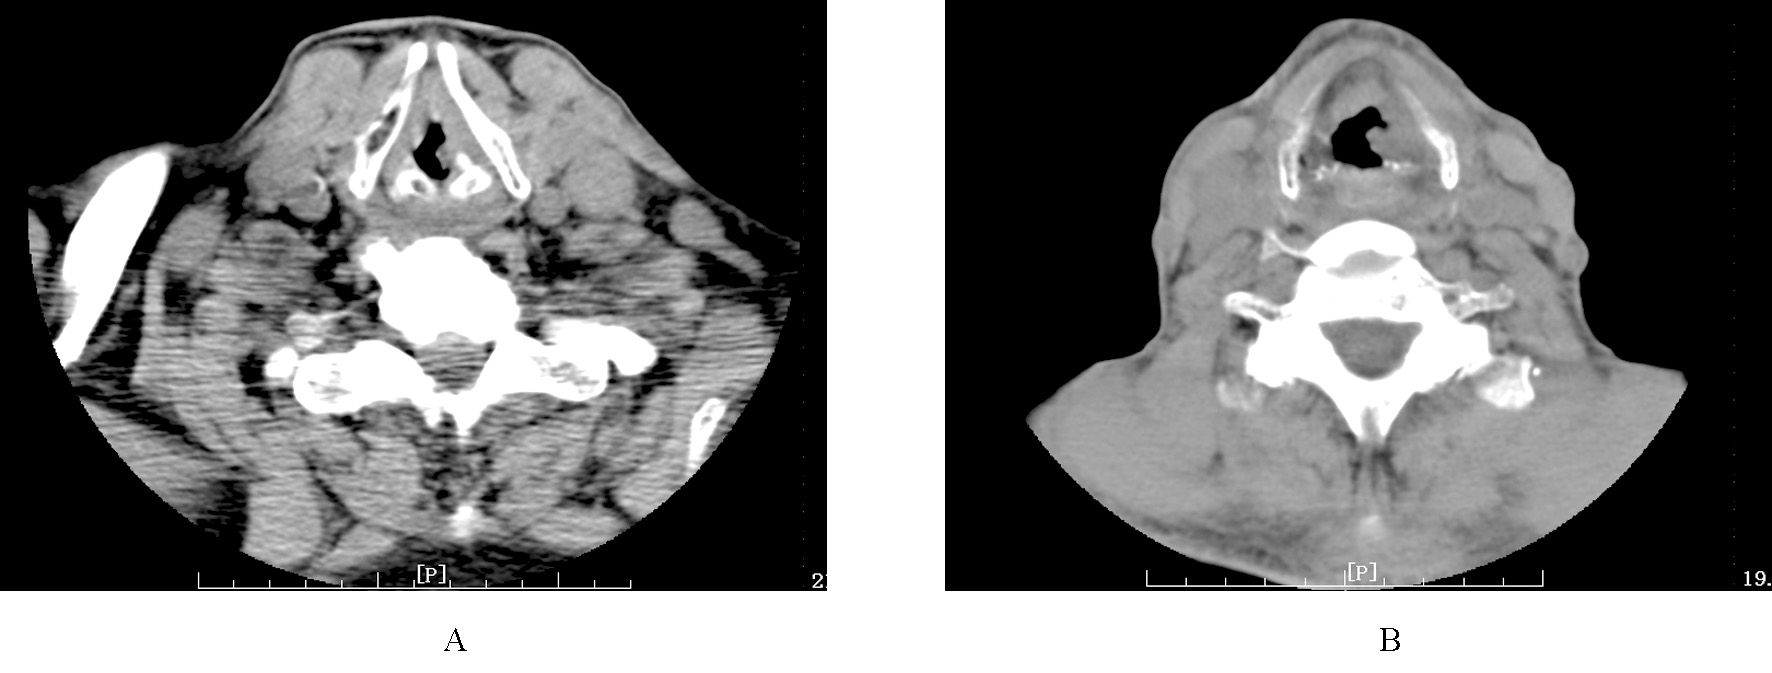
\includegraphics[width=.7\textwidth,height=\textheight,keepaspectratio]{./images/Image00152.jpg}
 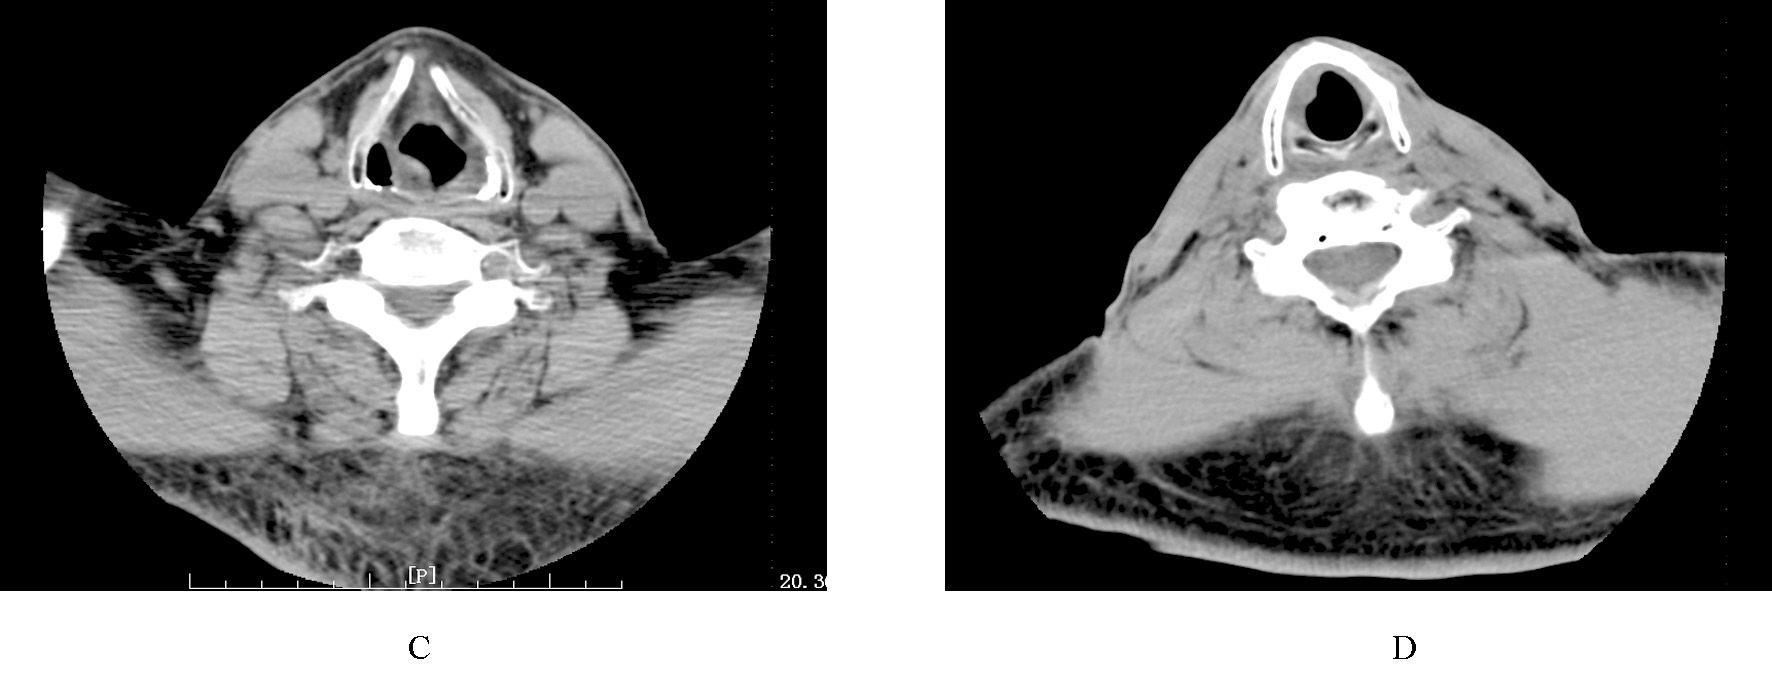
\includegraphics[width=.7\textwidth,height=\textheight,keepaspectratio]{./images/Image00153.jpg}
 \captionsetup{justification=centering}
 \caption{喉癌\\{\small A.左侧声带局部增厚突起;B.近左侧杓状会厌襞处局部软组织结节,突向喉前庭;C.右侧杓状会厌襞处局部软组织结节,突向喉前庭;D.环状软骨水平、右侧声带下局部软组织增厚}}
 \label{fig6-10}
  \end{figure} 

\textbf{【鉴别诊断】}

1.喉息肉:与早期局限于声带表面的癌肿在影像学上很难鉴别,主要依靠病理组织学来判断。当声带癌向深部浸润使喉旁间隙缩小或消失时,两者鉴别不难。

2.喉结核:以往认为本病好发于20~40岁年轻者,而近期报道老年患者也不少见。喉结核病变较广泛,后期以瘢痕狭窄、畸形改变为主,喉支架一般保持完整。而喉癌常偏重于一侧,伴有软骨破坏。

3.喉咽癌:原发于杓会厌襞内侧的声门上型喉癌可使杓会厌襞增厚,梨状窝外移、狭小,这与喉咽癌(梨状窝型)较难区分。但梨状窝癌向环后发展,使杓-颈或环-颈间距增宽,有助于与喉癌鉴别。

\protect\hypertarget{text00014.html}{}{}

